\documentclass[polish, twoside, 12pt]{mwart}
\usepackage[polish]{babel}
\usepackage{polski}
\usepackage[T1]{fontenc}
\usepackage[utf8]{inputenc}
\usepackage{pdfpages}
\usepackage{booktabs}
\usepackage{lscape}

\usepackage{hyperref}
\hypersetup{
    colorlinks,
    citecolor=black,
    filecolor=black,
    linkcolor=black,
    urlcolor=black
}
\usepackage{listings}

\usepackage{tabularx}
\usepackage{ltablex}
\newcolumntype{x}{p{4cm}}

\usepackage{tikz-qtree}

\usepackage{amsmath}

\usepackage{graphicx}
\graphicspath{ {../figures/} }

\let\stdsection\section
\renewcommand*{\section}{\clearpage\stdsection}
\emergencystretch=3em
\linespread{1.1}

\begin{document}

\includepdf{../templates/title-page}
 
\newpage

\tableofcontents

\newpage

\listoffigures
 
\listoftables

\newpage

\section{Wstęp}

Czasom, w których aplikacje internetowe pisane były od podstaw z wykorzystaniem natywnych możliwości oferowanych przez połączenie technologii \emph{HTML}, \emph{CSS} oraz \emph{JavaScript} zdecydowanie daleko do współczesności. Aktualnie programiści do wyboru mają ogromny zbiór gotowych platform programistycznych służacych do tworzenia aplikacji internetowych w języku \emph{JavaScript}.

Podjęcie decyzji, którą platformę użyć może być bardzo trudne, a fakt jej wybrania może mieć poważne konsekwencje w przyszłości z powodu kilku potencjalnych problemów. Jednym z takich problemów może sytuacja, w której popularna i szeroko rekomendowana przez społeczność programistów biblioteka traci na popularności z powodu nowego konkurenta. Konkurent ten oferuje wszystkie najbardziej lubiane cechy wcześniejszej biblioteki, przy okazji pozbywa się pewnych wad, a dodatkowo wprowadza swoje własne pomysły, czy też usprawnienia. Aktualnie wykorzystywana biblioteka przestaje być utrzymywana, w przypadku ujawnienia się luki związanej z bezpieczeństwem nie pojawia się tzw. łatka (ang. \emph{patch}). Programiści są wtedy zmuszeni do migracji do nowej biblioteki, bądź też do samodzielnego utrzymywania powoli wymierającej bilioteki.

Migracja może posiadać różny stopień skomplikowania. W idealnej sytuacji programiści podmieniają jedynie bibliotekę na inną, która zachowuje w pełni kompatybilny interfejs. Do takiej sytuacji możemy porównać wejście biblioteki \emph{React} \cite{react} w wersji \emph{16.0}, w której to implementacja głównego rdzenia została przepisana od podstaw, przy okazji nie wprowadzając zmian w interfejsie. Z drugiej strony można przytoczyć przykład bibliteki \emph{AngularJS} \cite{angularjs} oraz swojego następny o podobnej nazwie \emph{Angular} \cite{angular}. Pomimo podobieństwa w nazwie różnice są bardzo drastyczne i bibliotekę \emph{Angular} należy analizować jako zupełnie osobny byt.

Pomiędzy bibliotekami z rodziny \emph{Angular}, a \emph{React} aktualnie głównym konkurentem jest platforma \emph{Vue.js}, która czerpie garściami z lubianych oraz sprawdzonych funkcjonalności swoich konkurentów.

Jedną z mniej popularnych bibliotek jest \emph{mithril.js}. Chwali się on bardzo małą objętością oraz wysoką wydajnością w porównaniu do swoich konkurentów.

Celem pracy jest porównanie pięciu platform programistycznych służących do tworzenia aplikacji internetowych. Są to \emph{Angular}, \emph{AngularJS},
\emph{mithril.js}, \emph{React} oraz \emph{Vue.js}. Porównanie zostanie przeprowadzone pod kątem wydajności czasowej oraz pamięciowej. Uzyskane wyniki pomóc mogą programistom zadecydować z jakiej biblioteki skorzystać jeśli ważnym elementem jest ich wydajność.

Praca składa się z dziesięciu rozdziałów. Rozdział pierwszy stanowi wstęp. W rozdziale drugim przedstawiono sformułowanie problemu. Rozdział trzeci zawiera opis środowiska przeglądarki internetowej, sposób jej działania oraz wykorzystywane technologie. W rozdziale czwartym opisano format danych o nazwie \emph{Trace Event Fomat}. Rozdział piąty zawiera opis zbioru narzędzi o nazwie \emph{Chrone DevTools}. Rozdział szósty przedstawia specyfikacje aplikacji pomagających przy badaniach przeprowadzanych w ramach pracy magisterskiej. W rozdziale siódmym znajduje się opis poszczególnych plaform programistycznych oraz implementacji stworzonych za ich pomocą. Rozdział ósmy zawiera przeprowadzone badania oraz osiągniete wyniki. W rozdziale dziewiątym zawarto porównanie wyników oraz wysunięte wnioski. Ostatni, dzięsiaty rozdział stanowi podsumowanie.

\section{Specyfikacja problemu}

Aby w trakcie badań wydajnościowych uzyskać wyniki, które będzie można ze sobą porównywać wszystkie biblioteki będą implementowały taki sam schemat aplikacji.

Aplikacja będzie składać się z nastepujących elementów dla każdej implementacji niezależnie od biblioteki:

\begin{enumerate}
  \item Inicjalizacja głównego komponentu/modułu - każda z bibliotek musi zostać zainicjalizowana, dzięki czemu zostanie wyrenderowany pierwszy komponent lub zostanie uruchomiony główny moduł odpowiedzialny za dalsze renderowanie.
  \item Główny komponent - korzystając z biblioteki musi być zaimplementowany główny komponent, który odpowiedzialny będzie za pobranie listy elementów potrzebnych do wyrenderowania oraz zgłoszenia potrzeby aktualizacji tej listy. Główny komponent przekazywać będzie listę elementów do komponentu odpowiedzialnego za wyświetlenie elementów w tablicy.
  \item Komponent tablicy elementów - komponent ten odpowiedzialny będzie za wyświetlenie stuktury tabeli, w której poszczególne wiersze odpowiadać będą elementom tablicy. Komponent musi reagować na zmiany elementów w tablicy i wyświetlać różnice najszybciej jak tylko jest w stanie to zrobić.
\end{enumerate}

Aby przykładowa aplikacja bardziej przypominała przypadek ze świata rzeczywistego tablica przechowywać będzie elementy, które symulować będą stany wirtualnych maszyn. Na stan maszyny składać będą się takie parametry jak aktualne wykorzystanie procesora, aktualne wykorzystanie pamięci, aktualne wykorzystanie dysku, czas ciągłej pracy. W pojedyńczym wierszu tablicy będą również wyświetlane dane, które nie będą się zmieniać w czasie takie jak nazwa wirtualnej maszyny, całkowita dostępna pamięć, całkowita dostępna przestrzeń na dysku. Pozwoli to bibliotekom implementującym mechanizm wirtualnego obiektowego modelu dokumentu na wykorzystanie swoich zalet i ponowne użycie fragmentów \emph{DOM}, aby zminimalizować czas potrzebny do aktualizacji widoku.

Kod odpowiedzialny za generowanie tablicy oraz aktualizowanie ich elementów jest współdzielony pomiędzy wszystkimi bibliotekami, więc narzut czasowy oraz pamięciowy powinien być taki sam i nie powinien powodować przekłamań w uzyskanych wynikach badań.

\section{Środowisko przeglądarki internetowej}

Przeglądarka internetowa (ang. \emph{web browser}) to program komputerowy służący do pobierania i wyświetlania stron internetowych udostępnianych przez serwery \emph{WWW} (ang. \emph{World Wide Web}). Komunikacja z serwerem odbywa się najczęściej za pomocą protokołu \emph{HTTP} (ang. \emph{Hypertext Transfer Protocol}) lub odpowiednika w wersji szyfrowanej \emph{HTTPS} (ang. \emph{Hypertext Transfer Protocol Secure}). Nierzadko przeglądarki internetowe są w stanie obsługiwać inne protokoły takie jak np. \emph{FTP} (ang. \emph{File Transfer Protocol}) wykorzystywany do serwerów plików, czy też protokoły \emph{POP3} (ang. \emph{Post Office Protocol}), \emph{IMAP} (ang. \emph{Internet Message Access Protocol}) i \emph{SMTP} (ang. \emph{Simple Mail Transfer Protocol}) wykorzystywane do poczty elektronicznej. 

\subsection{Technologie}

Współczesne strony internetowe to produkty, które powstały z połączenia wielu różnych technologii. Technologie te muszą być bardzo dobrze wspierane i obsługiwane przez przeglądarki internetowe. Działając razem pozwalają dostarczyć wysokiej jakości doświadczenia dla użytkownika (ang. \emph{User experience}). 

\subsubsection{HTML 5.1} \label{html}

Hipertekstowy język znaczników (ang. \emph{HyperText Markup Language}) to język służący do określenia struktury strony internetowej. Definicję \emph{HTML 5.1} stanowi \emph{W3C REC-HTML51} \cite{w3c-rec-html51}. Oprócz głównego tekstu \emph{HTML} zawiera tak zwane znaczniki, które zawierają dodatkowe informacje pozwalające przeglądarce internetowej odpowiednio zinterpretować określony fragment strony interetowej. Za pomocą znaczników możemy formować fragmenty strony w takie struktury takie jak hiperłącza, akapity, listy, nagłówki, czy też formularze. Znaczniki najczęściej występują w parach (jako znacznik otwierając oraz zamykający) definiując zakres swojego działania.

\lstinputlisting[language=HTML, caption=Przykładowa prosta strona internetowa z formularzem, label={lst:example-page}]{../examples/html.html}

W listingu \ref{lst:example-page} przedstawiono bardzo krótką, przykładową, lecz w pełni poprawną i funkcjonalną stronę internetową. Strona internetowa zaczyna się od \emph{<!DOCTYPE html>}. Jest to specjalny znacznik, który musi być umieszczony jako pierwszy. Informuje on przeglądarkę o tym, że tekst jest w formacie \emph{HTML}. Kolejnym znacznikiem jest \emph{html} z atrybutem \emph{lang}, jest to główny znacznik, będacy korzeniem całej zagnieżdzonej struktury. Atrybut \emph{lang} informuje przeglądarkę internetową o języku, dla którego strona jest dedykowana. Kolejnym znacznikiem jest znacznik \emph{head} zawierający infomację o systemie kodowania (w tym wypadku jest to  kodowanie \emph{UTF-8}) oraz tytuł strony. Może on zawierać dodatkowe metadane opisujące stronę internetową. Z punktu widzenia użytkownika najważniejszym fragmentem jest znacznik \emph{body}, który zawiera właściwą treść, czyli w tym przypadku jest to głównie formularz \emph{form}. Dwa najważniejsze atrybuty opisujące formularz to \emph{action} informujący przeglądarkę gdzie wysłać dane wpisane przez użytkownika oraz \emph{method} na podstawie, którego przeglądarka wie jaką metodę protokołu HTTP zastosować. Przykładowy formularz zawiera jedno pole tekstowe \emph{input type="text"} oraz jedno pole do wpisywania haseł \emph{input type="password"}. Hasło wpisane w tego typu pole jest domyślnie ukryte przez przeglądarkę dla celów bezpieczeństwa. Oba pola dodatkowo opisane są etykietami \emph{label}. Ostatnim nieopisanym jeszcze znacznikiem jest \emph{button type="{}submit"}, który wyświetlany jest jako przycisk służący do wysłania formularza. Każda przeglądarka posiada wbudowany zestaw styli, który definiuje wygląd każdego znacznika przewidzianego w dokumentacji \emph{HTML 5}. Rysunek \ref{fig:example-page-chrome} przedstawia przykładową stronę wyrenderowaną w przeglądarce internetowej \emph{Chrome}.

\begin{figure}[ht]
  
\includegraphics[width=\textwidth]{html-chrome.png}
  \caption{Przykład wyrenderowany w przeglądarce Chrome}
  \label{fig:example-page-chrome}
\end{figure}

\subsubsection{CSS 3}

Kaskadowe arkusze stylów (ang. \emph{Cascading Style Sheets}) to język służący do opisu wyświetlania struktury opisanej w języku \emph{HTML}. Wersja 3 składa się z wielu modułów. Każdy z nich dodaje nowe możliwości lub rozszerza te zdefiniowane w CSS 2 zachowując wsteczną kompatybilność (ang. \emph{backward compatibility}).

\begin{enumerate}
  \item css3-background - specyfikacja \emph{W3C REC-CSS3-Background} \cite{w3c-rec-css3-background}
  \item css3-box - specyfikacja \emph{W3C REC-CSS3-Box} \cite{w3c-rec-css3-box}
  \item css-cascade-3 - specyfikacja \emph{W3C REC-CSS-Cascade-3} \cite{w3c-rec-css3-cascade}
  \item css3-color - specyfikacja \emph{W3C REC-CSS3-Color} \cite{w3c-rec-css3-color}
  \item css3-content - specyfikacja \emph{W3C REC-CSS-Content-3} \cite{w3c-rec-css3-content}
  \item css-fonts-3 - specyfikacja \emph{W3C REC-CSS-Fonts-3} \cite{w3c-rec-css3-fonts}
  \item css3-gcpm - specyfikacja \emph{W3C REC-CSS-GCPM-3} \cite{w3c-rec-css3-gcpm}
  \item css3-layout - specyfikacja \emph{W3C REC-CSS-Template-3} \cite{w3c-rec-css3-template}
  \item css3-mediaqueries - specyfikacja \emph{W3C REC-CSS3-Mediaqueries} \cite{w3c-rec-css3-mediaqueries}
  \item css3-multicol - specyfikacja \emph{W3C REC-CSS3-Multicol} \cite{w3c-rec-css3-multicol}
  \item css3-page - specyfikacja \emph{W3C REC-CSS3-Page} \cite{w3c-rec-css3-page}
  \item css3-selectors - specyfikacja \emph{W3C REC-CSS3-Selectors} \cite{w3c-rec-css3-selectors}
  \item css-3-ui - \emph{W3C REC-CSS-UI-3} \cite{w3c-rec-css3-ui}
\end{enumerate}

Za pomocą \emph{CSS} opisać można wszystkie pojęcia odpowiedzialne za reprezentację elementów \emph{HTML}, takie jak rodzina czcionek, kolor tekstu, marginesy, czy też pozycja danego elementu względem innych elementów lub okna przeglądarki.

\emph{CSS} został stworzony w celu odseparowania struktury dokumentu od formy jego prezentacji. Zalety tej separacji to zwiększony zakres dostępności witryny, zmniejszona zawiłość dokumentu, łatwiejsze wprowadzanie zmian w strukturze dokumentu. \emph{CSS} ułatwia także zmiany w wyświetlaniu strony w zależności od obsługiwanego medium (ekran komputera, ekran tabletu, ekran telefonu komórkowego).

Arkusz stylów składa się z reguł określających styl dla wybranych elementów dokumentu. Reguła składa się z selektora oraz deklaracji. Selektor określa grupę elementów, którego ma dotyczyć deklaracja. Deklaracja określa formatowanie i składa się z nazwy jednej z właściwości i jej wartości napisanej po dwukropku. Deklaracja musi być otoczona nawiasami klamrowymi.

\begin{lstlisting}
selektor { 
	wlasciwosc: wartosc; 
}
\end{lstlisting}

Selektory oraz deklaracje można grupować. Zgrupowane selektory rozdziela się przecinkami, natomiast deklaracje średnikami.

\begin{lstlisting}
selektor, selektor2 { 
	wlasciwosc1: wartosc1;
	wlasciwosc2: wartosc2;
}
\end{lstlisting}

Selektory mogą poszukiwać elementy na podstawie wielu różnych wartośći, jedne z nich to:

\begin{itemize}
  \item nazwa elementu np. \emph{h1},
  \item atrybut \emph{class} elementu np. \emph{.my-class},
  \item identyfikator elementu, czyli atrybut \emph{id} np. \emph{\#element-id},
  \item połączenie wcześniejszych selektorów operatorem logicznym \emph{OR} np. \emph{h1.my-class},
  \item połączenie wcześniejszych selektorów operatorem logicznym \emph{AND} np. \emph{\#element-id .my-class}.
\end{itemize}

Dobrą praktyką jest definiowanie selektorów na podstawie atrubutu \emph{class}, natomiast identyfikator, czyli atrybut \emph{id} powinien służyć do jednoznacznej identyfikacji elementu w strukturze \emph{HTML}. Zgodnie z dokumentacją wiele znaczników może posiadać taką samą klasę, natomiast identyfikator aby spełniał swoje zadanie musi być unikalny.

Ponieważ standardowy wygląd znaczników jest bardzo prosty to dodatkowo nieostylowane strony internetowe zdarzają się bardzo rzadko. W celu pokazania jak duża może być różnica pomiędzy standardowym, a specjalnie ostylowanym wyglądem strony internetowej rysunek \ref{fig:example-page-mithril} przedstawia poprzedni przykład strony z formularzem wzbogacony o bardzo lekką bibliotekę \emph{CSS} o nazwie \emph{Milligram} \cite{milligram}. Biblioteka ta jest bardza lekka, jej rozmiar wynosi tylko 2kB.

\begin{figure}[ht]
  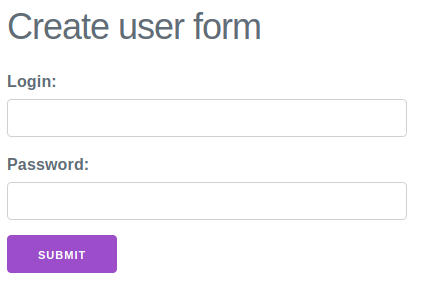
\includegraphics[width=\textwidth]{html-css-chrome.png}
  \caption{Ostylowany przykład wyrenderowany w przeglądarce Chrome}
  \label{fig:example-page-mithril}
\end{figure}

\subsubsection{JavaScript}

\emph{JavaScript} to skryptowy język programowania, stworzony przez firmę Netscape, najczęściej stosowany na stronach internetowych. Pod koniec lat 90. XX wieku organizacja \emph{ECMA} wydała na podstawie JavaScriptu standard języka skryptowego o nazwie \emph{ECMAScript}. Najnowsza stabilna wersja \emph{ECMAScript} nosi nazwę \emph{ECMAScript 2016} \cite{es2016} i została wydana 17 czerwca 2016. Wersja ta często występuje pod nazwą \emph{ECMAScript 5} pomimo iż jest to forma odradzana i organizacja ECMA zapowiedziała, że stabilna wersja tego standardu będzie ogłaszana co rok i to właśnie rok wydania będzie oficjalnie odpowiadał numerowi wersji. 

Najczęściej spotykanym zastosowaniem języka JavaScript są strony \emph{WWW}. Skrypty napisane w tym języku najczęściej służą do zapewnienia interaktywności poprzez odpowiednie reagowanie na zdarzenia generowane przez użytkownika. Skrypty JavaScriptu uruchamiane przez strony internetowe mają znacznie ograniczony dostęp do komputera użytkownika. 

Platformy programistyczne, które zostaną zbadane w ramach pracy magisterskiej napisane są języku JavaScript. Wspomagają one proces pisania aplikacji internetowej dostarczając odpowiednich funkcji i organizująć strukturę strony internetowej zgodnie z wytycznymi konkretnej platformy programistycznej.

W języku \emph{HTML} za umieszczanie skryptów \emph{JavaScript} odpowiedzialny jest znacznik \emph{script} z opcjonalnymi parametrami \emph{type="text/javascript"} i \emph{language="javascript"}.

\emph{JavaScript} może zostać użyty również poza środowiskiem przeglądarki internetowej dzięki darmowemu środowisku uruchomieniowemu \emph{Node.js} \cite{node.js}. \emph{Node.js} zaprojektowany został do tworzenia wysoce skalowalnych aplikacji internetowych, szczególnie serwerów napisanych w języku \emph{JavaScript}. Architektura \emph{Node.js} składa się z silnika \emph{V8} \cite{v8} stworzonego przez Google i opiera się na sterowaniu zdarzeniami wykorzystującymi asynchroniczny system wejścia-wyjścia. Kod źródłowy jest otwarty (ang. \emph{open source}) i każdy może brać udział w jego rozwijaniu. Domyślnym menedżerem pakietów dla \emph{Node.js} jest \emph{Npm} \cite{npm}, jednak warto zapoznać się z alternatywnym rozwiązaniem o nazwie \emph{Yarn} \cite{yarn}. \emph{Yarn} oferuje szybsze pobieranie zależności, większe bezpieczeństwo poprzez dodatkowe sprawdzanie sum kontrolnych oraz bardziej płaska stuktura drzewa pobranych zależności.

\subsubsection{DOM} \label{dom}

Obiektowy model dokumentu (ang. \emph{Document Object Model}) to zespół klas i interfejsów programistycznych umożliwiających dostęp do elementów strony napisanej w języku \emph{HTML}. Istnieje kilka tzw. poziomów \emph{DOM} (ang. \emph{level}):

\begin{enumerate}
  \item DOM Level 0 - nie stanowi oficjalnego standardu \emph{W3C} \cite{w3c}, pierwotnie był modelem zaimplementowanym w przeglądarce Netscape Navigator 3.0, obecnie wspierają go wszystkie przeglądarki.
  \item DOM Level 1 - specyfikacja \emph{W3C REC-DOM-Level-1} \cite{w3c-rec-dom-level-1}.
  \item DOM Level 2 - specyfikacja \emph{W3C REC-DOM-Level-2} \cite{w3c-rec-dom-level-2}.
  \item DOM Level 3 - definicję stanowi sześć specyfikacji.
  \begin{itemize}
    \item DOM Level 3 Core - specyfikacja \emph{W3C DOM-Level-3-Core} \cite{w3c-rec-dom-level-3-core}.
    \item DOM Level 3 Load and Save - specyfikacja \emph{W3C DOM-Level-3-LS} \cite{w3c-rec-dom-level-3-ls}.
    \item DOM Level 3 XPath - specyfikacja \emph{W3C DOM-Level-3-XPath} \cite{w3c-rec-dom-level-3-xpath}.
    \item DOM Level 3 Views and Formatting - specyfikacja \emph{W3C DOM-Level-3-Views} \cite{w3c-rec-dom-level-3-views}.
    \item DOM Level 3 Requirements - specyfikacja \emph{W3C DOM-Level-3-Requirements} \cite{w3c-rec-dom-level-3-requirements}.
    \item DOM Level 3 Validation - specyfikacja \emph{W3C DOM-Level-3-Val} \cite{w3c-rec-dom-level-3-val}.
  \end{itemize}
\end{enumerate}

\emph{DOM} pozwala dokonywać dowolnych modyfikacji poprzez tworzenie, usuwanie i modyfikację tzw. węzłów (ang. \emph{nodes}). Początkowo nie istniał standardowy obiektowy model dokumentu. Twórcy najpopulaniejszych przeglądarek tworzyłi własne niezgodne ze sobą modele. Organizacja \emph{W3C} \cite{w3c} przygotowała ujednolicony standard obiektowego modelu dokumentu, w którym dokment jest dostępny pod postacią globalnego obiektu \emph{document}, który posiada metody do np. pobierania elementu na podstawie identyfikatora \emph{document.getElementById} lub na podstawie klasy \emph{document.getElementByClassName}. Standard \emph{W3C} definiuje interfejsy \emph{DOM} tylko dla języków \emph{JavaScript} i \emph{Java}.

Rysunek \ref{fig:example-page-dom} przedstawia drzewo \emph{DOM} wygenerowane dla wcześniejszej przykładowej strony internetowej opisanej w punkcie \ref{html}.

\begin{figure}
  \centering
  \begin{tikzpicture}
    \Tree[.html 
      [.head 
        [.meta ]
        [.title ]
      ]
      [.body 
        [.h2 ]
        [.form 
            [.label ]
            [.input ]
            [.label ]
            [.input ]
            [.button ]
        ]
      ]
    ]
  \end{tikzpicture}
  \caption{Przykładowe drzewo \emph{DOM}}
  \label{fig:example-page-dom}
\end{figure}

\subsubsection{CSSOM} \label{cssom}

Obiektowy model kaskadowych arkuszy stylów (ang. \emph{CSS Object Model}) to zespół interfejsów programistycznych umożliwiających dostęp do stylów napisanych w języku \emph{CSS}.

\emph{CSSOM} blokuje wszystko przed wyświetleniem tzn. przeglądarka internetowa nie zacząć renderować dopóki w pełni nie zostanie zakończona budowa \emph{CSSOM}. W przypadku nieoptymalnej struktury \emph{CSS} budowa może trwać bardzo długo co skutkuje widoczną dla użytkownika białą stroną bez zawartości.

\emph{CSSOM} musi być zbudowany na nowo z każdym przeładowaniem strony, oznacza to, iż nawet jeśli pliki \emph{CSS} zostały umieszczone w pamięci podręcznej (ang. \emph{cache}) to nie uchroni to przeglądarki przed koniecznością budowy \emph{CSSOM}.

Istnieje związek pomiędzy kaskadowymi arkuszami stylów, które przeglądarka ładuje i skryptami \emph{JavaScript} umieszczonymi na stronie. Żeby przeglądarka wyświetliła cokolwiek musi poprawnie zakończyć budowę \emph{CSSOM}, w przypadku gdy budowa ta zostanie wstrzymana przez skrypty czas potrzebny na wyświetlenie jakiegokolwiek elementu wzrośnie. W przypadku nieoptymalnej kombinacji skryptów oraz stylów czas ten może wzrosnąc drastycznie skutkując bardzo negatywnymi doświadczeniami użytkownika, w najgorszym wypadku spowodować zniechęcenie użytkownika do dalszego oczekiwania i opuszczenie strony.

Rysunek \ref{fig:example-page-cssom} przedstawia drzewo \emph{CSSOM} wygenerowane dla przykładu opisanego w punkcie \ref{html}.

\begin{figure}
  \centering
  \resizebox{\textwidth}{!}{
    \begin{tikzpicture}
      \Tree[.body(font-size:10px) 
        [.h1(font-size:1.6rem) ]
        [.form(font-size:1.4rem) 
          [.label(font-size:1.2rem) ]
          [.input(font-size:1.2rem) ]
        ]
        [.button(font-size:1.4rem) ]
      ]
    \end{tikzpicture}
  }
  \caption{Przykładowe drzewo \emph{CSSOM}}
  \label{fig:example-page-cssom}
\end{figure}
\subsubsection{HTTP/1.1} \label{http/1.1}

Protokół przesyłania dokumentów hipertekstowych (ang.\emph{(Hypertext Transfer Protocol)}) to protokół za pomocą którego przysła się żadania udostępnienia dokumentów z serwera \emph{WWW} oraz informacje z forumlarzy internetowych. Obecną definicję \emph{HTTP} stanowi \emph{RFC 2616} \cite{rfc2616}

Protokół \emph{HTTP} udostępnia znormalizowany sposób komunikowania się komputerów ze sobą. Określa on formę żądań (ang. \emph{requests}) klienta dotyczących danych oraz formę odpowiedzi (ang. \emph{responses}) serwera na te żądania. Klientem może być np. przeglądarka internetowa.  \emph{HTTP} jest zaliczany do protokołów bezstanowych (ang. \emph{stateless}) ponieważ nie zachowuje żadnych informacji o poprzednich transakcjach z klientem. Pozwala to znacznie zmniejszyć obciążenie serwera, jednak uniemożliwia zapamiętanie konkretnego stanu użytkownika w sytuacji gdy jest to potrzebne np. przy implementacji koszyka z zakupami w sklepie internetowym. Najczęstszym rozwiązaniem tego problemu jest wprowadzenie mechanizmu ciasteczek (ang. \emph{cookies}). Ciasteczka to mały fragment tekstu zawierający pary klucz-wartość. Przesyłane są one z każdym żądaniem do serwera. Alternatywne rozwiązania to ukryte parametry (gdy aktualna strona zawiera formularz) oraz parametry umieszczone w ujednoliconym formacie adresowania zasobów (ang. \emph{Uniform Resource Locator}.

Wywołania protokołu \emph{HTTP} zaczynają się od \url{http://}. \emph{HTTP} standardowo korzysta z portu numer 80 protokołu kontroli transmisji (ang. \emph{Transmission Control Protocol}).

Zapytanie \emph{HTTP} zaczynaja się od nazwy metody, która określa akcję jaką obiekt tworzący zapytanie chce wykonać na zasobie podstępnym pod określonym adresem. Dostępne metody to:

\begin{enumerate}
  \item \emph{GET} - pobranie zasobu.
  \item \emph{HEAD} - pobranie informacji o zasobie, metoda stosowana do sprawdzania dostępności zasobu.
  \item \emph{PUT} - aktualizacja zasobu.
  \item \emph{POST} - stworzenie nowego zasobu.
  \item \emph{DELETE} - usunięcie zasobu.
  \item \emph{OPTIONS} - pobranie informacji o możliwych operacjach do wykonania na zasobie.
  \item \emph{TRACE} - metoda stosowana do diagnostyki kanału komunikacyjnego.
  \item \emph{PATCH} - częściowa aktualizacja zasobu.
\end{enumerate}

Listing \ref{lst:http-request} przestawia przykładowe żądanie \emph{HTTP/1.1} przeglądarki Chrome. Listing \ref{lst:http-response} przedstawia odpowiedź na przykładowe żądanie.

\begin{lstlisting}[caption=Przykładowe żądanie \emph{HTTP/1.1}, label={lst:http-request}]
GET / HTTP/1.1
Host: localhost:8080
Connection: keep-alive
Pragma: no-cache
Cache-Control: no-cache
Upgrade-Insecure-Requests: 1
User-Agent: Mozilla/5.0 (X11; Linux x86_64) AppleWebKit/537.36 
  (KHTML, like Gecko) Chrome/60.0.3112.90 Safari/537.36
Accept: text/html,application/xhtml+xml,application/xml;q=0.9,
  image/webp,image/apng,*/*;q=0.8
Accept-Encoding: gzip, deflate, br
Accept-Language: pl-PL,pl;q=0.8,en-US;q=0.6,en;q=0.4
\end{lstlisting}

\begin{lstlisting}[caption=Przykładowa odpowiedź \emph{HTTP/1.1}, label={lst:http-response}]
HTTP/1.1 200 OK
X-Powered-By: Express
Content-Type: text/html; charset=utf-8
Content-Length: 116
ETag: W/"74-IGpXmXtcB0E/yn+QbK3UFXMrMU8"
Date: Tue, 15 Aug 2017 10:28:41 GMT
Connection: keep-alive
\end{lstlisting}

\subsubsection{HTTPS} \label{https}

Bezpieczny protokół przesyłania dokumentów hipertekstowych (ang. \emph{Hypertext Transfer Protocol Secure}) to szyfrowana wersja protokołu \emph{HTTP}. Obecną definicję \emph{HTTPS} stanowi \emph{RFC 2660} \cite{rfc2660}

W odróżnieniu od protokołu \emph{HTTPS}, protokół \emph{HTTP} do komunikacji stosuje niezaszyfrowany tekst. HTTPS początkowo szyfrował dane za pomocą protokołu \emph{SSL} (ang. \emph{Secure Socket Layer}), natomiast obecnie używany jest protokół \emph{TLS} (ang. \emph{Transport Layer Security}). Szyfrowanie zapobiega przechwytywaniu i zmienianiu przesyłanych danych. 

Wywołania protokołu \emph{HTTPS} zaczynają się od \url{https://}. \emph{HTTPS} standardowo korzysta z portu numer 443 protokołu kontroli transmisji. 

\subsubsection{HTTP/2} \label{http/2}

Protokół \emph{HTTP/2} to unowocześniejszego protokołu \emph{HTTP/1.1}. Został on opracowany na podstawie wczesnych wersji ekperymentalnego protokołu \emph{SPDY} \cite{spdy}. Obecną definicję \emph{HTTP/2} stanowi \emph{RFC 7540} \cite{rfc7540}. W przeciwieństwie do wersji \emph{HTTP/1.1}, protokół \emph{HTTP/2} jest w pełni binarny. Format podobny do tekstu zrozumiałego dla człowieka zastąpiony został zbiorem tak zwanych ramek (ang. \emph{frames}) o ściśle określonym formacie i zastosowaniu. Poniżej przedstawiono najważniejsze zalety protokołu \emph{HTTP/2}.

\begin{enumerate}
  \item \emph{Multipleksowanie} - protokół nawiązuje tylko jedno trwałe połączenie z serwerem za pomocą którego pobierane są wszystkie pliku niezbędne do prawidłowego wyświetlenia strony.
  \item \emph{Powiadomienia Push} - serwer może wysłać dodatkowe informacje np. może wysłać pliki, które są potrzebne do prawidłowego wyświetlenia strony zanim przeglądarka internetowa zauważy tą potrzebę i ją zgłosi.
  \item \emph{Ustalanie priorytetów} - każde zapytanie o plik posiada swój priorytet, który nadawany jest przez serwer. Umożliwia to najpierw pobranie najważniejszych plików, które pozwolą wyrenderować kluczowe fragmenty strony internetowej, a następnie doczytać kolejne elementy.
  \item \emph{Kompresja nagłówków} - protokół \emph{HTTP/2} unika duplikacji informacji występującyh pomiędzy różnymi nagłówkami i wysyła je w skompresowanym formacie.
  \item \emph{Szyfrowanie} - pomimo, iż szyfrowanie według protokołu \emph{HTTP/2} nie jest wymagane to większość najważniejszych przeglądarek internetowych implementuje \emph{HTTP/2} wyłącznie z wykorzystaniem protokołu \emph{TLS}.
\end{enumerate}

\subsection{Proces wyświetlania strony internetowej}

Końcowym produktem przeglądarki internetowej jest w pełni załadowana i wyrenderowana strona internetowa, która oferuje użytkownikowi wszystkie zaimplementowane wcześniej funkcjonalności. Proces, który jest odpowiedzialny za dostarczenie tego produktu można podzielić na cztery etapy.

\begin{enumerate}
  \item pobieranie.
  \item parsowanie.
  \item budowanie.
  \item renderowanie.
\end{enumerate}

\subsubsection{Pobieranie}

Proces ładowania strony internetowej w przeglądarce zaczyna się od pobrania treści strony internetowej wraz ze wszystkimi zasobami potrzebnymi do jej wyświetlenia.
Przeglądarka pobiera wszystkie elementy za pomocą żądań \emph{HTTP}. Użytkownik może rozpocząć pobieranie poprzez:

\begin{enumerate}
  \item wpisanie adresu strony internetowej.
  \item kliknięcie na odnośnik przekierowujący do innej strony lub do podstrony aktualnej strony internetowej.
  \item przeładowanie aktualnej strony internetowej.
\end{enumerate}

Moment stworzenia pierwszego żądania równoznaczny jest z początkiem ładowania strony internetowej. Od tego momentu przeglądarka może zacząć zbierać dodatkowe informacje na temat wydajności np. o całkowitym czasie ładowania strony. Przeglądarka internetowa tworzy żądanie zgodnie z zasadami protokołu \emph{HTTP/1.1}, który został bardziej szczegółowo opisny w punkcie \ref{http/1.1}. Jeśli serwer wspiera obsługę nowszej wersji \emph{HTTP/2} wtedy wykorzystany jest nowszy protokół opisany w punkcie \ref{http/2}. Całe wykonanie żądania przez przeglądarkę możemy podzielić na poszczególne fazy:

\begin{enumerate}
  \item \emph{Kolejkowanie} - przeglądarka kolejkuje żądania w przypadku gdy:
    \begin{itemize}
      \item aktualnie istnieją inne żądania do przetworzenia o wyższym priorytecie.
      \item aktualnie istnieje już sześć otwartych połączeń TCP dla konkretnego źródła (ang. \emph{origin}). Ograniczenie to dotyczy tylko \emph{HTTP/1.0} oraz \emph{HTTP/1.1}.
    \end{itemize}
  \item \emph{Odroczenie} - żądanie czeka na swoją kolej na przetworzenie z przyczyn wymienionych we wcześniejszym podpunkcie.
  \item \emph{Podgląd DNS} - przeglądarka stara się przetłumaczyć adres internetowy na adres \emph{IP} za pomocą usługi systemu nazw domenowych (ang. \emph{Domain Name System}).
  \item \emph{Negocjowanie z pośrednikiem} - przeglądarka prowadzi negocjacje z serwerem pośredniczącym (ang. \emph{proxy}).
  \item \emph{Wysłanie żądania} - przeglądarka wysyła żądanie do serwera.
  \item \emph{Oczekiwanie} - przeglądarka oczekuje na pierwsze bajty odpowiedzi, w tym czasie mierzony jest parametr TTFB (ang. \emph{Time To First Byte}) oznaczający czas jaki minął zanim przeglądarka otrzymała pierwszy bajt odpowiedzi.
  \item \emph{Pobieranie zawartości} - przeglądarka pobiera całą zawartość odpowiedzi.
  \item \emph{Otrzymanie notyfikacji Push} - serwer wysyła dodatkowe dane dla przeglądarki, jest to element unikalny dla \emph{HTTP/2}.
  \item \emph{Czytanie notyfikacji Push} - przeglądarka czyta oraz interpretuje otrzymane wcześniej dodatkowe dane.
\end{enumerate}

Rysunek \ref{fig:request-timing-chrome} wygenerowany został za pomocą \emph{Chrome DevTools}. Pozwala on w bardzo prosty sposób dokonać analizy czasu trwania poszczególnych faz przetwarzania żądania.

\begin{figure}[ht]
  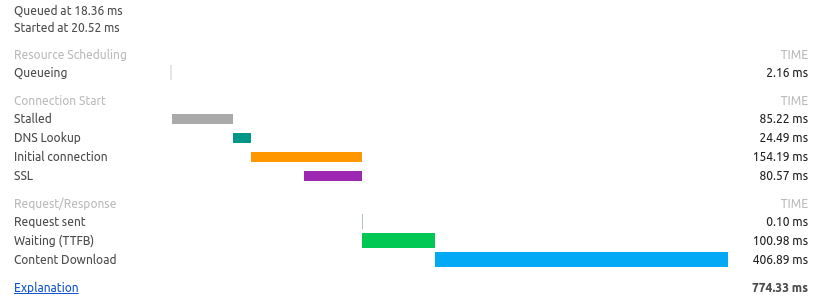
\includegraphics[width=\textwidth]{request-timing-chrome.png}
  \caption{Przykładowy widok przedstawiający czas trwania poszczególnych faz przetwarzania żądania}
  \label{fig:request-timing-chrome}
\end{figure}

\subsubsection{Parsowanie}

W momencie gdy przeglądarka w pełni przetworzy żądanie i otrzyma dokument w postaci pliku zawierającego kod \emph{HTML} wtedy następuje proces czytania treści tego pliku w procesie zwanym parsowaniem. Pod pojęciem parsowanie ukrywa się czytanie treści z uwzględnieniem analizy składniowej specyficznej dla konkretnego języka. W przypadku języka \emph{HTML} przeglądarka oczekuje poprawnie zdefiniowanych znaczników z właściwymi parametrami. 

Jeśli przeglądarka napotka znacznik odnoszący się do kolejnego zasobu wtedy proces parsowania zostaje zatrzymany i tworzone jest żądanie  w celu pobrania zawartości potrzebnej do pełnego wyświetlenia strony. Dopiero gdy przeglądarka pobierze cały zewnętrzny zasób proces parsowania zostaje kontynuowany. Znaczniki blokujące poprzez tworzenie odniesienia do zewnętrznego zasobu to:

\begin{enumerate}
  \item załączenie pliku ze stylami CSS.
  \item załączenie pliku z kodem w języku JavaScript.
  \item załączenie pliku graficznego.
\end{enumerate}

Listingi \ref{lst:include-css}, \ref{lst:include-js}, \ref{lst:include-img} przedstawiają przykładowe znaczniki tworzące odniesienia do zewnętrznych zasobów.

\begin{lstlisting}[caption=Przykładowe załączenie pliku ze stylami \emph{css}, label={lst:include-css}]
<link rel="stylesheet" type="text/css" href="style.css">
\end{lstlisting}

\begin{lstlisting}[caption=Przykładowe załączenie pliku z kodem w języku \emph{JavaScript}, label={lst:include-js}]
<script type="text/javascript" src="script.js">
\end{lstlisting}

\begin{lstlisting}[caption=Przykładowe załączenie pliku graficznego, label={lst:include-img}]
<img src="image.png">
\end{lstlisting}

\subsubsection{Budowanie}

W chwili, w której przeglądarka zakończy parsowanie dokumentu i wszystkie zewnętrzne zasoby zostaną pobrane następuje proces budowania strony, czyli łączenia informacji znalezionych w głównym pliku \emph{HTML} oraz pobranych zasobach. Na budowę strony składają się trzy kroki:

\begin{enumerate}
  \item \emph{Konstrukcja DOM} - obiektowa reprezentacja struktury opisanej w pliku \emph{HTML}. Szerzej opisana w punkcie \ref{dom}.
  \item \emph{Konstrukcja CSSOM} - obiektowa reprezentacja kaskadowych arkuszy stylów. Szerzej opisana w punkcie \ref{cssom}.
  \item \emph{Konstrukcja drzewa renderowania (ang. Render Tree)} - drzewiasta struktura będąca połączeniem \emph{DOM} oraz \emph{CSSOM}, na podstawie którego przeglądarka jest w stanie poprawnie wyświetlić stronę internetową.
\end{enumerate}

\subsubsection{Renderowanie}

Po wykonaniu wszystkich wcześniejszych kroków przeglądarka jest w końcu gotowa przejść do procesu renderowania. Większość współczesnych urządzeń odświeża ekran z częstotliwością 60 razy na sekundę. Jeśli aktualnie wykonywana jest jakaś animacja, przesuwanie lub użytkownik zwyczajnie przewija stronę internetową wtedy przeglądarka musi dopasować się do częstotliwości odświeżania urządzenia i przygotować nowy obrazek lub klatkę (ang. \emph{frame}) dla każdego pojedynczego odświeżenia ekranu. Każda z tych klatek posiada 16 milisekund na przygotowanie się do wyświetlenia. Wynika to z bardzo prostego obliczenia:

\begin{equation}
  \frac{1s}{60} = 16.66 ms
\end{equation}

Należy jednak pamiętać o tym, że przeglądarka posiada również swoje zadania do wykonania dlatego w rzewczywistości warto wykonać wszystkie własne zadania w czasie ponizej 10 milisekund. Po przekroczeniu tej wartości spada częstotliwość wyświetlania klatek co może objawiać się efektem migotania elementów wyświetlanych na ekranie. Migotanie jest niechcianym zjawiskiem ponieważ odbija się bardzo negatywnie na doświadczeniach użytkownika korzystającego ze strony internetowej.

Proces renderowania możemy podzielić na pięć postępujących po sobie etapów tzw. rurociągu (ang. \emph{pipeline}). Każdy z tych etapów ma znączacy wpływ na to w jaki sposób wyświetlone zostaną piksele na ekranie.

\begin{enumerate}
  \item \emph{JavaScript / CSS} - język \emph{JavaScript} może zostać użyty do zadań, które ostatecznie skutkują wizualnymi zwianami na ekranie. Do tego typu zadań możemy zaliczyć np. wywołanie animacji, sortowanie zestawu danych, dodawanie elementów do strony za pomocą interfejsów \emph{DOM}. Animacje mogą również być definiowane za pomocą kasakdowych arkuszy styli.
  \item \emph{Kalkulacja styli} - służy do określenia które reguły \emph{CSS} zaaplikować do konkretnych elementów na podstawie pasujących selektorów oraz oblicza wartości poszczególnych właściwości \emph{CSS}.
  \item \emph{Układ (ang. Layout)} - na tym etapie przeglądarka wie już co wyświetlić na podstawie \emph{DOM}, wie też w jaki sposób to wyświetlić na podstawie \emph{CSSOM} oraz zna relację pomiędzy tymi dwoma elementami na podstawie \emph{Render Tree}. Na tym etapie przeglądarka oblicza jak dużą przestrzeń elementy będą zajmować na ekranie. Obliczenia te są potrzebne ponieważ właściwości jednego elementu często wpływają relatywnie na inne. Przykładowo szerokość elementu \emph{body}, które umiejscowione jest bardzo wysoko blisko korzenia w drzewie elementów wpłynie na szerokość wszystkich podelementów aż do tzw. liści. Z racji dużej ilości obliczeń proces ten może mocno angażować procesor.
  \item \emph{Malowanie (ang. Paint)} - malowanie jest processem wypełniania poszczególnych pikseli na ekranie. Sprowadza się do wyświetlenia tekstu, kolorów, obrazków, obramowań, cieni, czyli głównie wszystkiego co wpływa na wizualną część każdego elementu. Najczęściej elementy malowane są na wielu powierzchniach popularnie nazywanych warstwami.
  \item \emph{Kompozycja (ang. Compositing)} - ponieważ elementy strony mogły zostać potencjalnie namalowane na wielu różnych warstawach, przeglądarka musi wyświetlić warstwy w odpowiedniej kolejności. Dotyczy to szczególnie elementów, które wzajemnie na siebie nachodzą, od błędnej kompozycji może zależeć czy element, który powinien być przykryty przypadkowo zostanie wyrysowany na warstwie znajdującej się na samej górze.
\end{enumerate}

Każda część rurociągu może potencjalnie wywołać efekt migotania dlatego też ważne jest dokładne zrozumienie jest co powoduje wyzwalanie poszczególnych części.

Czasami można spotkac się z określeniem rasteryzacji (ang. \emph{rasterization}) używanym jako synonim etapu malowania. Dzieję się tak dlatego ponieważ malowanie składa się z dwoch zadań:

\begin{enumerate}
  \item tworzenia listy prymitywnych elemtów do wyrysowania takich jak np. punkty, odcinki, krzywe, okręgi, koła, kwadraty.
  \item wypełniania pikseli na ekranie.
\end{enumerate}

To właśnie ostatnie z wymienionych zadań jest właściwą rasteryzacją, czyli działaniem polegającym na jak najwierniejszym przedstawieniu płaskiej figury geometrycznej na urządzeniu rastrowym, dysponującym skończoną rozdzielczością, w naszym przypadku na ekranie urządzenia. Warto przytoczyć tutaj fakt, iż niektóre implementacje wykonują wymienione zadania na różnych wątkach procesora (ang. \emph{threads}), jednak dzieje się to poza jakąkolwiek kontrolą programisty.

Przygotowanie klatki do wyświetenia nie zawsze musi przechodzić przez wszystkie pięć etapów rurociągu. Istnieją trzy kombinacje elementów, które odgrywają rolę przy przygotowaniu klatki w momencie gdy nastąpiła wizualna zmiana obojętnie czy z powodu kodu napisanego w języku \emph{JavaScript}, czy też z powodu zdefiniowanych styli \emph{CSS}.

\begin{enumerate}
  \item \emph{JavaScript / CSS > Style > Layout > Paint > Composite} - pełne przejście przez wszystkie etapy. Ma miejsce w momencie gdy zmienia się właściwość powiązana z układem elementów na stronie np. szerokość, wysokość, pozycja elementu. Przeglądarka musi sprawdzić wszystkie pozostałe elementy, dokonać odpowiednich obliczeń potrzebnych na pełne przemalowanie warstw, a ostatecznie dokonać ich kompozycji.
  \item \emph{JavaScript / CSS > Style > Paint > Composite} - kombinacja ta ma miejsce w momencie gdy zmienia się właściwość powiązana wyłącznie z malowaniem strony jak np. tło, kolor tekstu. Przeglądarka nie musi wtedy na nowo opracowywać układu strony, co nie zmienia faktu, że musi przejść przez etap malowania.
  \item \emph{JavaScript / CSS > Style > Composite} - najbardziej pożądana kombinacja ponieważ nie wymaga ani opracowania układu strony, ani jej przemalowania. Ma miejsce tylko gdy zmienia się właściwość nie powiązana ze wcześniej wymienionymi etapami.
\end{enumerate}

\subsection{Model współbieżności oraz pętla zdarzeń}

Język JavaScript posiada model współbieżności oparty na pętli zdarzeń (ang. \emph{event loop}). Ten model różni się od modeli zaimplementowanych w innych językach jak np. \emph{C} lub \emph{Java}.

Poniższe sekcje wyjaśniają model teoretyczny. Nowoczesne silniki JavaScript implementują i optymalizują opisaną tutaj semantykę.

\subsubsection{Stos}

Wywołania funkcji tworzą ramki (ang. \emph{frames}), które odkładane są na strukturze danych o nazwie stos(ang. \emph{stack}).

\begin{lstlisting}
function foo(b) {
  var a = 1;
  return a + b;
}

function bar(x) {
  var y = 1;
  return foo(x * y);
}

console.log(bar(2));
\end{lstlisting}

Na przedstawionym przykładzie w momencie wywołania funkcji \emph{bar} zostaje utworzona pierwsza ramka przechowująca argumenty przekazane do tej funkcji oraz lokalne zmienne. Następnie gdy wewnątrz funkcji \emph{bar} wywoływana jest funkcja \emph{foo} tworzona jest druga ramka przechowująca te same informacje tj. przekazane argumenty oraz lokalne zmienne. Ramka umieszczana jest na samej górze stosu nad pierwszym elementem. Kiedy następuje powrót z funkcji \emph{foo} element na samej górze stosu zostaje zdjęty (pozostawiając tylko ramkę powiązaną z wywołaniem funkcji \emph{bar}). Po powrocie z funkcji \emph{bar} stos powonie staje się pusty.

\subsubsection{Sterta}

Obiekty utworzone w języku JavaScript są umieszczane w stercie (ang. \emph{heap}). Poprzez stertę rozumi się dużą w większości nieustrukturyzowaną przestrzeń pamięci.

\subsubsection{Kolejka}

Środowisko wykonawcze języka JavaScript zawiera kolejkę (ang. \emph{queue}), która składa się z wiadomości do przetworzenia. Funkcja jest przypisana do odpowiedniej wiadomości. W momencie gdy stos posiada wystarczająco dużo miejsca wiadomość jest pobierana z kolejki i przetwarzana. Przetwarzanie polega na wywołaniu skojarzonej funkcji, a tym samym utworzeniu początkowej ramki stosu.
Przetwarzanie wiadomości kończy się, gdy stos staje się pusty.

\subsubsection{Pętla zdarzeń}

Pętla zdarzeń uzyskała swoją nazwę ze względu na to, jak zwykle jest to implementowana. Działanie pętli zdarzen obrazuje poniższy pseudokod:

\begin{lstlisting}
while (queue.waitForMessage()) {
  queue.processNextMessage();
}
\end{lstlisting}

Fragment \emph{queue.waitForMessage()} oczekuje synchronicznie, aż pojawi się wiadomość w kolejkce. Pętla zdarzen posiada kilka bardzo ważnych własności:

\begin{enumerate}
  \item \emph{Działanie do końca} - każda wiadomość jest przetwarzana całkowicie przed przetworzeniem jakiejkolwiek innej wiadomości. To zachowanie gwarantuje, iż raz wywołana funkcja będzie działać do końca przed uruchomieniem dowolnego innego kodu. Jako przykład innego działania można przedstawić język \emph{C}, gdzie np. jeśli funkcja dziąła w wątku może być zatrzymana w dowolnym momencie, aby uruchomić inny kod w innym wątku. Minusem tego modelu jest możliwość zaistnienia sytuacji w której przetwarzanie wiadomości trwa bardzo długo, w tym czasie aplikacja internetowa nie jest w stanie przetworzyć interakcji użytkownika. Przeglądarka obsługuje tą sytuację wyświetlając informację o tym, że wykonywanie skryptu trwa bardzo długo. Może to zniechęcić użytkownika do opuszczenia strony lub jej ponownego odświeżenia. Dobrą praktyką jest pisanie jak najkrótszej implementacji przetwarzania wiadomości.
  \item \emph{Sposób dodawania wiadomości} - w przeglądarce internetowej wiadomości dodawane są do kolejki w dowolnym momencie, w którym zdarzenie to ma miejsce pod warunkiem, że została dodana funkcja nasłuchująca konkretnego wydarzenia. Bez nasłuchiwania zdarzenia wiadomość ulega przepadnięciu. Istnieje możliwość dodanie wiadomości do kolejki za pomocą funkcji \emph{setTimeout}. Wiadomość ta zostanie dodana do kolejki po upływie czasu podanego jako argument funkcji. W przypadku, w którym w kolejce nie ma innej wiadomości to nowo dodana wiadomość zostanie przetworzona od razu, jeśli istnieją jakieś inne, wtedy komunikat dodany metodą \emph{setTimeout} będzie musiał poczekać zanim nie zostaną one przetworzone. Z tego powodu argument podany jako czas wkazuje na minimalny czas, a nie na gwarantowany czas. Z tego powodu należy również mieć na uwadze fakt, iż wywołanie funkcji \emph{setTimeout} z opóżnieniem 0 milisekund nie spowoduje przetworzena wiadomości od razu. Wszystko zależy od aktualnego stopnia zapełnienia kolejki.
  \item \emph{Brak blokowania} - w przeciwieńswie do wielu innych języków JavaScript nigdy się nie blokuje. Obsługa wejścia / wyjścia zazwyczaj odbywa się za pośrednictwem zdarzeń i wywołań zwrotnych. Tym samym gdy aplikacja nadal może przetwarzać inne rzeczy jak np. wprowadzanie danych przez użytkownika.
\end{enumerate}

\section{Trace Event Format} \label{trace-event-format-section}

Dane zebrane z przeglądarki internetowej podczas testów wydajnościowych zapisane zostały w formacie o nazwie \emph{Trace Event Format} \cite{trace-event-format}. Struktura \emph{Trace Event Format} zgodna jest ze standardem przechowywania danych JSON (ang. \emph{JavaScript Object Notation}) \cite{json} i może występować w dwóch wariantach.

\subsection{Wariant tablicowy}

Plik przechowujący dane w wariancie tablicowym (ang. \emph{JSON Array Format}) składa się z jednej tablicy przechowującej obikety zarejestrowanych zdarzeń. Zdarzenia te nie muszą być poukładane chronologicznie według znaczników czasu. Listing \ref{lst:example-table-variant} przedstawia przykładowy tablicowy wariant formatu \emph{Trace Event Format}.

\begin{lstlisting}[caption=Przykładowy wariant tablicowy, label={lst:example-table-variant}]
[{
  "name": "Asub",
  "cat": "PERF",
  "ph": "B",
  "pid": 22630,
  "tid": 22630,
  "ts": 829
}, {
  "name": "Asub",
  "cat": "PERF",
  "ph": "E",
  "pid": 22630,
  "tid": 22630,
  "ts": 833
}]
\end{lstlisting}

\subsection{Wariant obiektowy}

Plik przechowujący dane w wraciencie obiektowym (ang. \emph{JSON Object Format}) składa się z jednego, głównego obiektu. Obiekt ten może posiadać następujące pola:

\begin{enumerate}
  \item traceEvents - jedyne wymagane pole, które jest tablicą zarejestrowanych zdarzeń. Tablica ta odpowiada dokładnie wariantowi tablicowemu formatu \emph{Trace Event Format}.
  \item displayTimeUnit - jednostka, w której podane zostały znaczniki czasu. Możliwe jednostki to \emph{ms} oraz \emph{ns}. Domyślna jednostka to \emph{ms}.
  \item systemTraceEvents - ciąg znaków kompatybilnych z \emph{Linux ftrace} \cite{ftrace} lub \emph{Windows ETW} \cite{etw}.
  \item powerTraceAsString - ciąg znaków kompatybilnych z \emph{BattOr} \cite {battor}.
  \item stackFrames - struktura przechowująca informacje o ramkach odłożonych na stosie.
  \item samples - tablica przechowująca dane rozszerzające traceEvents o informacje zarejestrowane na poziomie systemu operacyjnego.
\end{enumerate}

Dopuszczona jest możliwość definicji pól o nazwach innych niż wymienione wcześniej dla dodatkowego opisania danych (metadane). Listing \ref{lst:example-object-variant} przedstawia przykładowy obiektowy wariant formatu \emph{Trace Event Format}.

\begin{lstlisting}[caption=Przykładowy wariant obiektowy, label={lst:example-object-variant}]
{
  "traceEvents": [[{
    "name": "Asub",
    "cat": "PERF",
    "ph": "B",
    "pid": 22630,
    "tid": 22630,
    "ts": 829
  }, {
    "name": "Asub",
    "cat": "PERF",
    "ph": "E",
    "pid": 22630,
    "tid": 22630,
    "ts": 833
  }],
  "displayTimeUnit": "ns",
}
\end{lstlisting}

\subsection{Zdarzenia}

Podstawowymi obiektami, które można poddać analizie są zdarzenia. Przykładowe, poprawne zdarzenie przedstawia listing \ref{lst:example-event}. Istnieje kilka rodzajów zdarzeń. Poniżej przedstawiono pola występujące w każdym zdarzeniu niezależnie od jego typu:

\begin{enumerate}
  \item name - nazwa zdarzenia.
  \item cat - kolekcja oddzielonych przecinkiem kategorii powiązanych ze zdarzeniem.
  \item ph - pojedynczy znak określający typ zdarzenia. Tablica \ref{tab:event-types} zawiera wszystkie prawidłowe wartości.
  \item ts - znacznik czasowy zdarzenia podany z dokładnością do milisekundy.
  \item tts - opcjonalny znacznik czasowy wątku zdarzenia podany z dokładnością do milisekundy.
  \item pid - identyfikator procesu, który spowodował zaistnienie zdarzenia.
  \item tid - identyfikator wątku, który spowodował zaistnienie zdarzenia.
  \item args - argumenty, które zostały dostarczone dla zdarzenia.
\end{enumerate}

\begin{center}
  \begin{tabularx}{\textwidth}{|X|X|}\hline
    \emph{Typ zdarzenia} & \emph{Fazy zdarzenia}\\ \hline
    Zdarzenia trwające (\emph{ang. duration events}) & \textbf{B} początek (\emph{ang. begin}),\newline
    \textbf{E} koniec (\emph{ang. end})\\ \hline
    Zdarzenia kompletne (\emph{ang. complete events}) & \textbf{X}\\ \hline
    Zdarzenia natychmiastowe (\emph{ang. instant events}) & \textbf{i, I}(przestarzałe)\\ \hline
    Zdarzenia zliczające (\emph{ang. counter events}) & \textbf{c}\\ \hline
    Zdarzenia asynchroniczne (\emph{ang. async events}) & \textbf{b} (początek),\newline
    \textbf{n} (natychmiastowe zdarzenie asynchroniczne),\newline
    \textbf{e} (koniec)\newline\newline
    \textit{Przestarzałe}\newline
    \textbf{S} (początek),\newline
    \textbf{T} (krok kolejny),\newline
    \textbf{p} (krok poprzedni),\newline
    \textbf{F} (koniec)\\ \hline
    Zdarzenia przepływające (\emph{ang. flow events}) & \textbf{s} (początek),\newline
    \textbf{t} (krok),\newline
    \textbf{f} (koniec)\\ \hline
    Zdarzenia obiektowe (\emph{ang. object events}) & \textbf{N} (stworzenie)\newline
    \textbf{O} (migawka)\newline
    \textbf{D} (zniszczenie)\\ \hline
    Zdarzenia z metadanymi (\emph{ang. metadata events}) & \textbf{M}\\ \hline
    Zdarzenia zrzutu pamięci (\emph{ang. memory dump events}) & \textbf{V} (zrzut pamięci globalnej)\newline
    \textbf{v} (zrzut pamięci procesu)\\ \hline
    Zdarzenia synchronizacji zegara (\emph{ang. clock sync events}) & \textbf{c}\\ \hline
    Zdarzenia kontekstowe (\emph{ang. context events}) & \textbf{(, )}\\ \hline
  \caption {Fazy zdarzeń i odpowiadające im typy}
  \label {tab:event-types}
  \end{tabularx}
\end{center}

Poniżej przedstawiono opis każdego z możliwych typów zdarzeń:

\begin{enumerate}
  \item zdarzenia trwające - umożliwiają określenie czasu trwania pracy nad danym wątkiem. Zdarzenia czasowe są określane przez typy \textbf{B} i \textbf{E}. Zdarzenie \textbf{B} musi nastąpić przed odpowiednim wydarzeniem \textbf{E}. Można zagnieżdżać zdarzenia \textbf{B} i \textbf{E}. Znaczniki czasowe dla zdarzeń muszą być ułożone w kolejności rosnącej dla danego wątku. Znaczniki czasu w różnych wątkach nie muszą być ułożone w kolejności rosnącej.
  \item zdarzenia kompletne - każde kompletne zdarzenie logicznie łączy parę zdarzeń (\textbf{B} i \textbf{E}). Kompletne zdarzenia są oznaczone przez typ fazy \textbf{X}.
  \item zdarzenia natychmiastowe - odpowiadają czemuś co miało miejsce lecz bez przypisanego czasu trwania.
  \item zdarzenia zliczające - mogą śledzić wartość lub wiele wartości zmieniających się w czasie.
  \item zdarzenia asynchroniczne - służą do rejestrowania asynchronicznych operacji. Mogą pochodzić zarówno z różnych procesów jak i wątków.
  \item zdarzenia przepływające - z założenia są bardzo podobne do zdarzeń asynchronicznych, ale dodatkowo pozwalają na łączenie ich ze sobą w wątkach i/lub procesach.
  \item zdarzenia obiektowe - służą za konstrukcję do śledzenia złożonych struktur danych.
  \item zdarzenia z metadanymi - są używane do powiązania dodatkowych informacji z wydarzeniami.
  \item zdarzenia zrzutu pamięci - odpowiadają zrzutom pamięci procesu lub grupie procesów.
  \item zdarzenia synchronizacji zegara - służą do synchonizacji czasu w przypadku gdy zdarzenia rejestrowane są przez różne byty.
  \item zdarzenia kontekstowe - są używane do oznaczania sekwencji zdarzeń.
\end{enumerate}

\begin{lstlisting}[caption=Przykładowe zdarzenie, label={lst:example-event}]
{
  "name": "myName",
  "cat": "category,list",
  "ph": "B",
  "ts": 12345,
  "pid": 123,
  "tid": 456,
  "args": {
    "someArg": 1,
    "anotherArg": {
      "value": "my value"
    }
  }
\end{lstlisting}

\section{Chrome DevTools}

Aplikacją, która znacząco wspomaga zbieranie informacji na temat wydajności czasowej jak i pamięciowej jest \emph{Chrome DevTools} \cite{chrome-devtools}. Jest to aplikacja wbudowana w przeglądarkę \emph{Chrome}. Zawiera szereg narzędzi do badania aplikacji internetowych oraz wizualizacji zebranych danych.

\subsection{Uruchamianie Chrome DevTools}

Aby uruchomić \emph{Chrome DevTools} wystarczy pobrać i uruchomić przeglądarkę \emph{Chrome} \cite{chrome}, a następnie wykonać dowolny z poniższych sposóbow:

\begin{itemize}
  \item Wybrać opcję \emph{Więcej narzędzi -> Narzędzia developerskie} z głównego menu przeglądarki \emph{Chrome},
  \item Kliknąc prawym przyciskiem myszki w dowolny element strony internetowej, a następnie wybrać opcję \emph{Inspekcja elementu},
  \item Wcisnąć kombinację przycisków \emph{Control+Shift+I}.
\end{itemize}

\subsection{Narzędzia Chrome DevTools}

\emph{Chrome DevTools} jest potężnym zbiorem narzędzi, na który składają się:

\begin{enumerate}
  \item Tryb urządzenia - wspomaga tworzenie stron internetowych z myślą o urządzeniach mobilnych takich jak np. smartfony. Korzystając z tego modułu możemy sprawdzić jak aplikacja zachowuje się przy różnych wielkościach ekranu, czy jest responsywna i czy pozwala bez przeszkód korzystać z funkcjonalności oferowanych przez stronę internetową. W trybie urządzenia możemy również emulować wbudowane w urządzenia czujniki jak np. GPS, czy też akcelerometr.
  \item Zakładka \emph{Elementy} - służy do modyfikacji w czasie rzeczywistym \emph{DOM} oraz \emph{CSS} pojedynczego wybranego elementu lub wielu zgrupowanych za pomocą selektora. Zakładka ta pozwala również dokonać inspekcji wszystkich animacji znajdujących się na stronie.
  \item Zakładka \emph{Konsola} - pozwala na wykonanie dowolnego poprawnego kodu \emph{JavaScript}. Z poziomu konsoli posiadamy dostęp do interfejsów \emph{DOM} i \emph{CSSOM} aktualnie załadowanej strony internetowej.
  \item Zakładka \emph{Źródła} - dzięki tej zakładce możemy debugować dowolny skrypt napisany w języku \emph{JavaScript}, który został załączony do strony internetowej. Dzięki wbudowanemu interfejsowi graficznemu w łatwy sposób możemy umieszczać punkty wstrzymania (ang. \emph{brakepoint}) i wykonywać kod linijka po linijce podglądając w czasie rzeczywistym wartość wszystkich zmiennych oraz ramek odłożonych na stos.
  \item Zakładka \emph{Sieć} - służy do podglądania zarówno wykresów czasowych ładowania poszczególnych elementów strony internetowej jak i nagłówków wszystkich żądań oraz odpowiedzi \emph{HTTP}.
  \item Zakładka \emph{Wydajność} - zakładka ta została bardziej szczegółowo opisana w następnym podrozdziale, ponieważ stanowi kluczowe narzędzie do celów badań wydajnościowych.
  \item Zakładka \emph{Pamięć} - służy do tworzenia migawki (ang. \emph{snapshot}) aktualnego stanu sterty. Pozwala również zbierać informacje o tym jak była alokowana pamięc komputerowa w trakcie działania aplikacji i reprezentować zebrane dane na wykresie czasowym.
  \item Zakładka \emph{Aplikacja} - dostarcza wglądu do takich elementów aplikacji internetowej jak manifest, ciasteczka, pamięc podręczna, lokalny magazyn (ang. \emph{local storage}), magazyn sesji (ang. \emph{session storage}). Dodatkowo pozwala modyfikować tworzyć oraz modyfikować istniejące wpisy w czasie rzeczywistym.
  \item Zakładka \emph{Bezpieczeństwo} - służy do rozwiązywania problemów związanych z certyfikatami internetowymi, za pomocą wbudowanej przeglądarki możemy zapoznać się ze szczegółowymi informacajami na temat każdego certyfikatu związanego ze stroną internetową.
\end{enumerate}

\subsection{Manualne zbieranie danych}
Aby manualnie zebrać dane na temat wydajności można wykorzystać zakładkę \emph{Wydajność (ang. Performance)}, która dostępna jest bezpośrednio po uruchomieniu \emph{Chrome DevTools}. Po wybraniu tej zakładki możemy zebrać dane na dwa sposoby:

\begin{enumerate}
  \item Klikając przycisk reprezentujący czarną kropkę przedstawiony na rysunku \ref{fig:chrome-devtools-performance-recording-runtime}. Spowoduje to nagrywanie (ang. \emph{recording}) wszelkich informacji od momentu wciśnięcia przycisku, strona internetowa jest już załadowana i uruchomiona w oknie przeglądarki. Nagrywanie należy zatrzymać klikając odpowiedni przycisk widoczny na ekranie. 
  \item Klikając przycisk reprezentujący kręcącą się strzałkę przedstawiony na rysunku \ref{fig:chrome-devtools-performance-recording-reload}. Spowoduje to przeładowanie strony internetowej i nagrywanie danych od samego początku procesu wczytywania strony internetowej aż do jej pełnego załadowania.
\end{enumerate}

\begin{figure}[ht]
  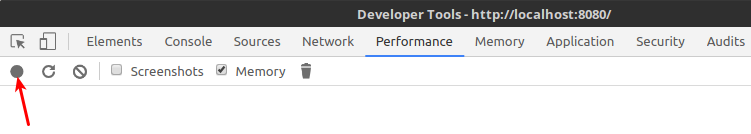
\includegraphics[width=\textwidth]{chrome-devtools-performance-recording-runtime.png}
  \caption{Nagrywanie danych w trakcie działania aplikacji}
  \label{fig:chrome-devtools-performance-recording-runtime}
\end{figure} 

\begin{figure}[ht]
  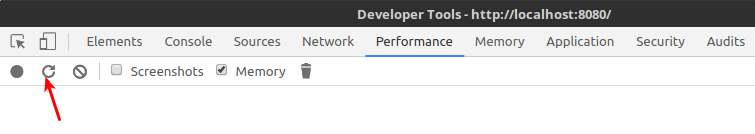
\includegraphics[width=\textwidth]{chrome-devtools-performance-recording-reload.png}
  \caption{Nagrywanie danych od momentu wczytywania strony}
  \label{fig:chrome-devtools-performance-recording-reload}
\end{figure}

\subsection{Wizualizacja zebranych danych}

Po zatrzymaniu nagrywania narzędzie automatycznie dokona reprezentacji zebranych danych za pomocą kilku widoków.

\subsubsection{Widok zbiorczy}

Najwyżej położonym widokiem służacym przedstwieniu zebranych danych jest widok zbiorczy przedstawiony na rysunku \ref{fig:chrome-devtools-performance-summary-view}, który składa się z kilku wykresów. Częścią wspólną wszystkich wykresów jest pozioma oś reprezentująca upływający czas. Poniżej opisane zostały wszystkie wykresy wchodzące w skład widoku zbiorczego:

\begin{enumerate}
  \item \emph{FPS} - wykres ten przedstawia ilość klatek na sekundę, które przeglądarka była w stanie przygotować do wyświetlenia.
  \item \emph{CPU} - wykres ten przedstawia zmieniające się w czasie zużycie procesora.
  \item \emph{NET} - wykres przedstawia czas, w którym przeglądarka pobierała wszystkie zasoby potrzebne do wyświetlenia strony oraz czekała na rozwiązanie wszelkich żądań \emph{HTTP}.
  \item \emph{HEAP} - wykres przestawiający ilość pamięci zajmowanej przez stertę. Bardzo dobrze widać na nim cykliczne działanie zbieracza nieużytków (ang. \emph{Garbage collector}), który jest jedną z metod automatycznego zarządzania dynamicznie przydzieloną pamięcią. Nagłe usuwanie ze sterty niepotrzebnych obiektów powoduje spadek na wykresie i powstawanie charakterystycznych "{}ząbków".
\end{enumerate}

\begin{figure}[ht]
  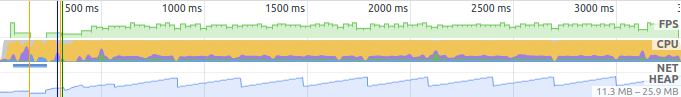
\includegraphics[width=\textwidth]{chrome-devtools-performance-summary-view.png}
  \caption{Przykładowy wygenerowany wykres zbiorczy}
  \label{fig:chrome-devtools-performance-summary-view}
\end{figure}

\subsubsection{Widok sieci}

Widok sieci przedstawiony na rysunku \ref{fig:chrome-devtools-performance-network-view} jest widokiem przedstawiającym w bardziej precyzyjny sposób odcinki czasu, w których ładowane były poszczególne zasoby.

\begin{figure}[ht]
  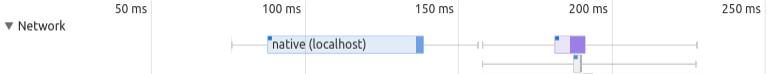
\includegraphics[width=\textwidth]{chrome-devtools-performance-network-view.png}
  \caption{Przykładowy wygenerowany widok sieci}
  \label{fig:chrome-devtools-performance-network-view}
\end{figure}

\subsubsection{Widok klatek}

Widok klatek przedstawiony na rysunku \ref{fig:chrome-devtools-performance-main-view} jest bardzo małym wykresem przedstawiającym jak zmieniała się liczba klatek na sekundę.

\begin{figure}[ht]
  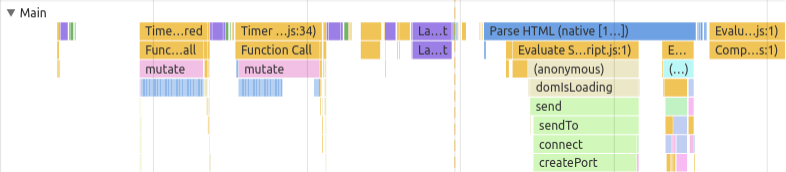
\includegraphics[width=\textwidth]{chrome-devtools-performance-main-view.png}
  \caption{Przykładowy wygenerowany widok klatek}
  \label{fig:chrome-devtools-performance-main-view}
\end{figure}

\subsubsection{Widok głównego wątku}

Widok głównego wątku przedstawiony na rysunku \ref{fig:chrome-devtools-performance-frames-view} pokazuje dokładnie jakie zadania były wykonywane przez główny wątek. Zadania te pogrupowane są w kategorie za pomocą kolorów:

\begin{enumerate}
  \item niebieski - obejmuje wszystkie zadania związane z ładowaniem zasobów (w tym parsowanie).
  \item żółty - obejmuje wszystkie zadania związane ze skrytami napisanymi w języku \emph{JavaScript}.
  \item fioletowy - obejmuje wszystkie zadania związane z renderowaniem.
  \item zielony - obejmuje wszystkie zadanie związane z malowaniem.
  \item szary - obejmuje wszystkie pozostałe zadanie nie wpasowujące się w pozostałe kategorie.
  \item biały - przedstawia okres bezczynności, w którym nie były wykonywane żadne zadania.
\end{enumerate}

Przyjęta kolorystyka jest spójna dla wszystkich widoków zakładki \emph{Wydajność}. Po wskazaniu kursorem myszki dowolnego elementu wyświetlone zostają bardziej szczegółowe informacje takie jak np. dokładny czas trwania zadania i jego źródło.

\begin{figure}[ht]
  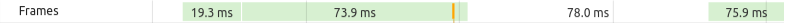
\includegraphics[width=\textwidth]{chrome-devtools-performance-frames-view.png}
  \caption{Przykładowy wygenerowany widok głównego wątku}
  \label{fig:chrome-devtools-performance-frames-view}
\end{figure}

\subsection{Manualne zbieranie danych pod kątek wydajności pamięciowej}

Aby manualnie zebrać dane na temat wydajności pamięciowej przed włączeniem nagrywania należy włączyć opcję zbierania informacji na temat zużycia pamięci, której położenie dokładnie przedstawione zostało na rysunku \ref{fig:chrome-devtools-performance-memory-checkbox}. Dzięki temu uzyskamy dostęp do jednego dodatkowego widoku wykorzystania pamięci.

\begin{figure}[ht]
  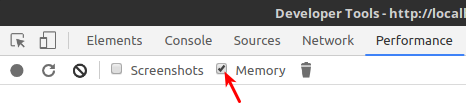
\includegraphics[width=\textwidth]{chrome-devtools-performance-memory-checkbox.png}
  \caption{Włączanie zbierania informacji na temat wykorzystania pamięci}
  \label{fig:chrome-devtools-performance-memory-checkbox}
\end{figure}

\subsubsection{Widok wykorzystania pamięci}

Widok wykorzystania pamięci przedstawiony na rysunku \ref{fig:chrome-devtools-performance-memory-view} pokazuje jak w czasie zmienia się ilość pamięci zajętej przez stertę. Dodatkowo wyświetla on najmniejszą i najwięszką liczbę elementów w następujących kategoriach:

\begin{enumerate}
  \item Dokumenty (ang. \emph{Documents}).
  \item Węzły (ang. \emph{Nodes}).
  \item Funkcje nasłuchujące (ang. \emph{Listeners}).
  \item Pamięc GPU (ang. \emph{GPU Memory}).
\end{enumerate}

\begin{figure}[ht]
  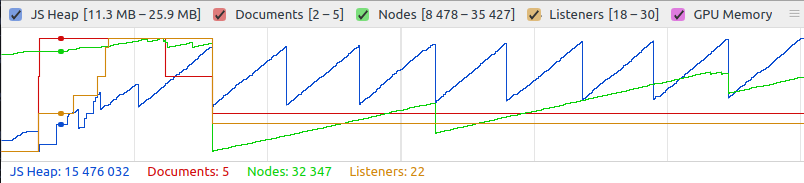
\includegraphics[width=\textwidth]{chrome-devtools-performance-memory-view.png}
  \caption{Przykładowy wygenerowany widok wykorzystania pamięci}
  \label{fig:chrome-devtools-performance-memory-view}
\end{figure}

\subsubsection{Zakładka \emph{Pamięć}}

\emph{Chrome DevTools} udostępnia specjalnie dedykowaną zakładkę o nazwie \emph{Pamięc}, która oferuje dodatkowe funkcjonalności przydatne przy np. debugowaniu aplikacji w celu znalezienia fragmentów kodu odpowiedzialnych za wyciek pamięci. Dostępne opcje to:

\begin{enumerate}
  \item migawka zawartości sterty - przedstawiona na rysunku \ref{fig:chrome-devtools-performance-heap-snapshot} pozwala utrwalić aktualny stan sterty, a następnie dokonać przeglądu jej zawartości za pomocą wbudowanej przeglądarki
  \item nagranie profilu alokacji pamięci - przedstawiona na rysunku \ref{fig:chrome-devtools-performance-allocation-profile} pozwala zbierać dane na temat alokacji pamięci z poziomu kodu napisanego w języku \emph{JavaScript}
  \item alokacja pamięci przedstawiona na wykresie czasowym - przedstawiona na rysunku \ref{fig:chrome-devtools-performance-allocation-timeline} pozwala zbierać dane na temat alokacji pamięci oraz automatycznie przedstawia je na osi czasowej
\end{enumerate}

Wszystkie opcje umożliwiają opcjonalne zapisanie zebranych danych do pliku na dysku.

\begin{figure}[ht]
  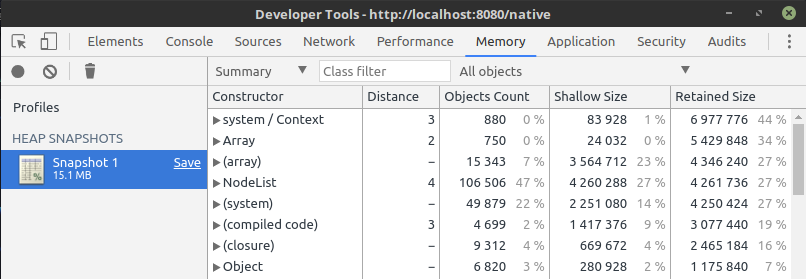
\includegraphics[width=\textwidth]{chrome-devtools-performance-heap-snapshot.png}
  \caption{Przeglądarka zawartości utworzonej migawki sterty}
  \label{fig:chrome-devtools-performance-heap-snapshot}
\end{figure}

\begin{figure}[ht]
  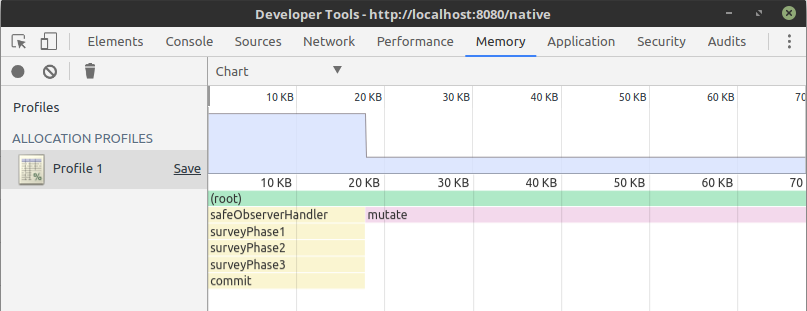
\includegraphics[width=\textwidth]{chrome-devtools-performance-allocation-profile.png}
  \caption{Wykres wygenerowany na podstawie profilu alokacji pamięci}
  \label{fig:chrome-devtools-performance-allocation-profile}
\end{figure}

\begin{figure}[ht]
  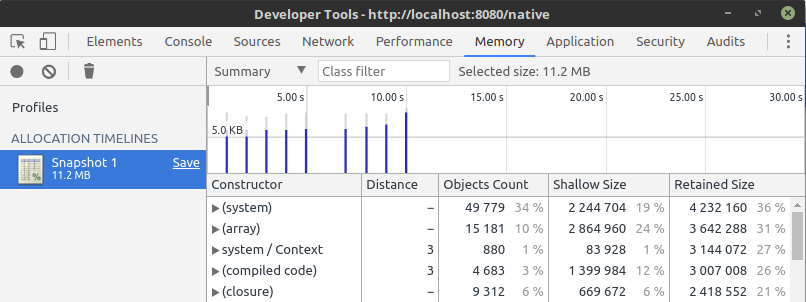
\includegraphics[width=\textwidth]{chrome-devtools-performance-allocation-timeline.png}
  \caption{Wykres czasowy alokacji pamięci}
  \label{fig:chrome-devtools-performance-allocation-timeline}
\end{figure}

\section{Aplikacje wspomagające badania}

W celu poprawnego przeprowadzenia badań zostały stworzone trzy małe aplikacje, które w znaczący sposób pomogły zebrać potrzebne dane. Głównym celem była automatyzacja wszystkich manualnych czynności. Osiągając cel główny udało się również zminimalizować efekt zniekształcenia pomiarów poprzez ręczną ingerencję człowieka.

\subsection{javascript-frameworks-benchmark}

\subsubsection{Opis}

\emph{javascript-frameworks-benchmark} to aplikacja, która przechowuje kod źródłowy wszystkich implementacji opartych na opisanych w pracy magisterskiej bibliotekach programistycznych. Po jej uruchomieniu pod lokalnym adresem \emph{http://localhost} i domyślnym porcie \emph{8080} dostępna jest strona za pomocą, której w łatwy sposób można przejść do wybranej przez siebie implementacji, co zostało przedstawione na rysunku \ref{fig:javascript-frameworks-benchmark}.

\begin{figure}[ht]
  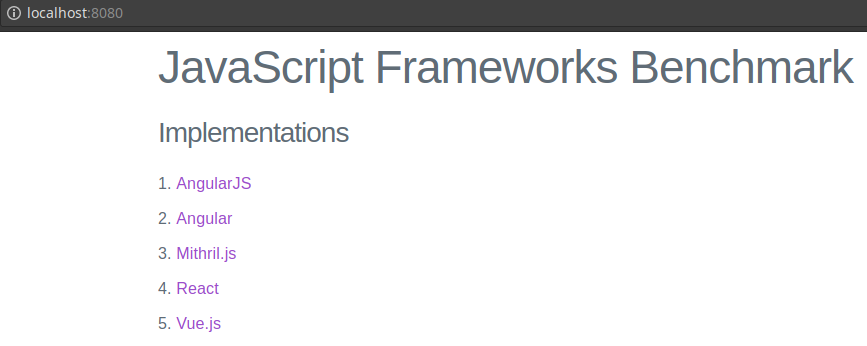
\includegraphics[width=\textwidth]{javascript-frameworks-benchmark.png}
  \caption{Widok strony wyboru implementacji}
  \label{fig:javascript-frameworks-benchmark}
\end{figure}

\subsubsection{Specyfikacja wewnętrzna}

Aplikacja została napisana w języku \emph{JavaScript} w standardzie \emph{ECMAScript 2016} \cite{es2016}. Środowiskiem uruchomieniowym jest \emph{Node.js} \cite{node.js} w wersji \emph{8.1.4}. Do poprawnego zainstalowania zewnętrznych zależności potrzebny jest menedżer pakietów \emph{Yarn} \cite{yarn}. Serwer obsługujący żadania \emph{HTTP} oparty został na bibliotece \emph{Express} \cite{express}.

\subsubsection{Specyfikacja zewnętrzna}

\textbf{Sposób uruchomienia programu} \newline

Żeby uruchomić program należy przejść za pomocą konsoli do głównego folderu programu a następnie wywołać następujące komendy:

\begin{lstlisting}
yarn install
yarn start
\end{lstlisting}

\textbf{Format danych wejściowych} \newline

Aplikacja nie przyjmuje danych wejściowych. \newline

\textbf{Format danych wyjściowych} \newline

Aplikacja nie podaje żadnych danych na wyjściu. Po uruchomieniu odpowiada na żądania \emph{HTTP} pod domyślnym adresem \emph{http://localhost:8080}

\subsection{chrome-performance-logs-recorder}

\subsubsection{Opis}

\emph{chrome-performance-logs-recorder} to aplikacja, która w automatyczny sposób uruchamia przeglądarkę internetową, przechodzi pod określony adres a następnie zbiera informacje związane z wydajnością aby pod koniec zapisać je do pliku z rozszerzeniem \emph{JSON} w formacie \emph{Trace Event Format}.

\subsubsection{Specyfikacja wewnętrzna}

Aplikacja została napisana w języku \emph{JavaScript} w standardzie \emph{ECMAScript 2016} \cite{es2016}. Środowiskiem uruchomieniowym jest \emph{Node.js} \cite{node.js} w wersji \emph{8.1.4}. Do poprawnego zainstalowania zewnętrznych zależności potrzebny jest menedżer pakietów \emph{Yarn} \cite{yarn} oraz przeglądarka internetowa \emph{Chrome}.

Automatyczne działanie opiera się na uruchomieniu serwera \emph{Selenium} \cite{selenium}, który to uruchamia a następnie podłącza się do przeglądarki internetowej. Po podłączeniu się do przeglądarki \emph{Selenium} udostępnia interfejs programistyczny do większości akcji, które może robić standardowy użytkownik przeglądarki. Aby korzystać w pełni z funkcjonalności oferowanych przez \emph{Selenium} użyto wiązań (ang. \emph{bindings}) dostarczanych przez paczkę \emph{wd} \cite{wd}, które pozwalają na dostęp do interfejsu \emph{Selenium} z poziomu języka \emph{JavaScript} w środowisku \emph{Node.js}.

\subsubsection{Specyfikacja zewnętrzna}

\textbf{Sposób uruchomienia programu} \newline

Żeby uruchomić program należy przejść za pomocą konsoli do głównego folderu programu a następnie wywołać następujące komendy:

\begin{lstlisting}
yarn install
yarn ./build/main.js [parametry]
\end{lstlisting}

\textbf{Format danych wejściowych} \newline

Aplikacja przyjmuje następujące parametry:

\begin{itemize}
  \item \emph{-{}-debug} (domyślna wartość \emph{false}) - flaga włączająca dodatkowe infomacje na wyjściu,
  \item \emph{-{}-duration} (domyślna wartość \emph{5000}) - czas zbierania informacji podanych w milisekundach,
  \item \emph{-{}-filter-event-names} (domyślna wartość \emph{' '}) - odseprowane przecinkami nazwy zdarzeń, o których informacje mają być zbierane przez aplikację,
  \item \emph{-{}-local-storage} (domyślna wartość \emph{key:value}) - pozwala zapisać w przeglądarce jedną parę klucz-wartość za pomocą mechanizmu przeglądarki \emph{LocalStorage},
  \item \emph{-{}-output-filename} (domyślna wartość \emph{'trace.json}) - nazwa pliku do którego mają zostać zapisane informacje,
  \item \emph{-{}-silent} (domyślna wartość \emph{false}) - flaga wyłączająca wszelkie informacje na wyjściu,
  \item \emph{-{}-trace-categories} (domyślna wartość \emph{'devtools.timeline,} \newline \emph{disabled-by-default-devtools.timeline.frame,rail'}) - odseparowane przecinkami kategorie zdarzeń, o których informacje mają być zbierane przez aplikację,
  \item \emph{-{}-trim} (domyślna wartość \emph{0}) - podana w procentach ilość zdarzeń, która ma zostać obcięta z końcowego raportu (na początku oraz na końcu),
  \item \emph{-{}-url} (domyślna wartość \emph{' '}) - adres strony internetowej, na podstawie której mają być zbierane przez aplikację informacje,
  \item \emph{-{}-verbose} (domyślna wartość \emph{false}) - flaga włączająca dodatkowe informacje na wyjściu.
\end{itemize}

\textbf{Format danych wyjściowych} \newline

Dane wyjściowe zapisywane są do pliku z rozszerzeniem \emph{JSON} oraz są zgodne z opisanym wcześniej formatem \emph
{Trace Event Format} [\ref{trace-event-format-section}].

\subsection{trace-event-format-analyzer}

\subsubsection{Opis}

\emph{trace-event-format-analyzer} to aplikacja, która potrafi dokonać analizy statystycznej danych zarejestrowanych w formacie \emph{Trace Event Format}.

\subsubsection{Specyfikacja wewnętrzna}

Aplikacja została napisana w języku \emph{JavaScript} w standardzie ECMAScript 2016 \cite{es2016}. Środowiskiem uruchomieniowym jest \emph{Node.js} \cite{node.js} w wersji \emph{8.1.4}. Do poprawnego zainstalowania zewnętrznych zależności potrzebny jest menedżer pakietów \emph{Yarn} \cite{yarn}.

Aplikacja wczytuje plik z rozszerzeniem \emph{JSON} a następnie iteruje po kolekcji zdarzeń dokonując odpowiednich obliczeń.

\subsubsection{Specyfikacja zewnętrzna}

\textbf{Sposób uruchomienia programu} \newline

Żeby uruchomić program należy przejść za pomocą konsoli do głównego folderu programu a następnie wywołać następujące komendy:

\begin{lstlisting}
yarn install
yarn ./build/main.js [parametry]
\end{lstlisting}

\textbf{Format danych wejściowych} \newline

Aplikacja przyjmuje następujące parametry:

\begin{itemize}
  \item \emph{-{}-complete-events} (domyślna wartość \emph{' '}) - odseparowane przecinkami nazwy zdarzeń kompletnych, które mają zostać poddane analizie,
  \item \emph{-{}-decimal-places} (domyślna wartość \emph{4}) - liczba miejsc po przecinku, do których mają zostać zaokrąglone wyniki,
  \item \emph{-{}-duration-events} (domyślna wartość \emph{' '}) - odseparowane przecinkami nazwy zdarzeń trwających, które mają zostać poddane analizie,
  \item \emph{-{}-immediate-events} (domyślna wartość \emph{' '}) - odseparowane przecinkami nazwy zdarzeń natychmiastowych, które mają zostać poddane analizie,
  \item \emph{-{}-output} (domyślna wartość \emph{'false}) - flaga włączająca zapis analizy do pliku w formacie \emph{JSON},
  \item \emph{-{}-paths} (domyślna wartość \emph{' '}) - odseparowane przecinkami ścieżki plików, które mają zostać wczytane oraz poddane analizie,
  \item \emph{-{}-silent} (domyślna wartość \emph{false}) - flaga wyłączająca wszelkie informacje na wyjściu,
  \item \emph{-{}-verbose} (domyślna wartość \emph{false}) - flaga włączająca dodatkowe informacje na wyjściu.
\end{itemize}

\textbf{Format danych wyjściowych} \newline

Dane wyjściowe, które opcjonalnie mogą zostać zapisane do pliku o rozszerzeniu \emph{JSON} są obiektem o następujących właściwościach:

\begin{enumerate}
  \item \emph{completeEvents} - obiekt zdarzeń kompletnych, którego właściwości odpowiadają nazwom analizowanych zdarzeń tego typu.
  \item \emph{durationEvents} - obiekt zdarzeń trwających, którego właściwości odpowiadają nazwom analizowanych zdarzeń tego typu.
  \item \emph{immediateEvents} - obiekt zdarzeń natychmiastowych, którego właściwości odpowiadają nazwom analizowanych zdarzeń tego typu.
\end{enumerate}

Każdy obiekt odpowiadający konkretnemu zdarzeniu posiada następujące właściwości:

\begin{enumerate}
  \item \emph{deltas} - przechowuje wyliczone statystyki na podstawie czasu pomiędzy kolejnymi zdarzeniami (jednostka to milisekundy).
  \item \emph{eps} - przechowuje wyliczone statystyki na podstawie ilości zdarzeń na sekundę (jednostka to zdarzenia na sekundę).
\end{enumerate}

Obiekt przechowujący wyliczone statystyki posiada następujace właściwości:

\begin{enumerate}
  \item \emph{min} - minimalna zarejestrowana wartość.
  \item \emph{mean} - średnia zarejestrowanych wartości.
  \item \emph{percentiles} - obliczone percentyle kolejno 50\%, 66\%, 75\%, 80\%, 85\%, 90\%, 95\%, 98\%, 99\%, 100\%.
  \item \emph{standardDeviation} - odchylenie standardowe.
  \item \emph{variance} - wariancja.
\end{enumerate}

\section{Platformy programistyczne do tworzenia aplikacji internetowych}

Aktualny wybór platform programistycznych do tworzenia aplikacji internetowych w języku \emph{JavaScript} jest bardzo szeroki. Zdecydowana większość bibliotek tworzona i utrzymywana jest zgodnie z zasadami wolnego oprogramowania \emph{Open Source}. Im większa popularność biblioteki tym większa szansa na wkład użytkowników w postaci nowych funkcjonalności, poprawiania błędów (w tym tych związanych z bezpieczeństwem), czy też optymalizacji. Podjęcie decyzji jakiej biblioteki użyć może być bardzo trudne zwłaszcza, że dosłownie z miesiąca na miesiąc może powstać nowa biblioteka zaskarbiająca sobie dużą sympatię programistów i tym samem pociągnać za sobą przepływ społeczeństwa zaangażowanego w tworzenie oprogramowania. Podstawowe porównanie bibliotek wraz z oferowanymi funkcjonalnościami przedstawione zostało w tabeli \ref{tab:frameworks-comparison}.

\subsection{Charakterystyczne funkcjonalności}

Współczesne biblioteki często wzajemnie zapożyczają i implementują pomysły, czy też rozwiązania, które sprawdziły się w środowisku produkcyjnym. Rozwiązania te pozwalają na szybkie tworzenie oprogramowania przez doświadczonego programistę, ale narzucona struktura oprogramowania jest na tyle prosta, że może nad nim pracować osoba mniej doświadczona programistycznie. Niektóre ze stosowanych roziązań niosą pozytywne efekty również dla użytkownika końcowego w postaci szybko renderującej się i reagującej na akcje użytkownika strony internetowej.

\subsubsection{Komponenty}

Architektura strony internetowej zbudowanej za pomocą współczesnych bibliotek programistycznych opiera się w zdecydowanej większości na idei komponentów. Poprzez komponenty rozumie się fragment strony internetowej, który posiada jasno określoną odpowiedzialność. Komponenty buduje się z połączenia \emph{HTML}, \emph{JavaScript} oraz \emph{CSS}, tym samym komponent zawiera wszystkie informacje potrzebne do wyświetlenia samego siebie oraz działania. Dzięki tej niezależności komponenty są w łatwy sposób testowalne, mają jasno określony interfejs za pomocą którego komunikują się z innymi komponentami. Raz określony komponent może być użyty w wielu miejscach co pozwala uniknąc niepotrzebnej duplikacji kodu.

Struktura strony internetowej opartej na komponentach może zostać przedstawiona za pomocą drzewa, którego korzeniem jest główny komponent, który najczęściej po prostu składa się z kilku komponentów o bardziej specyficznych odpowiedzialnościach. Te komponenty moga składać się z kolejnych i tak dalej. 

Komponenty mogą przechowywać swój aktualny stan potrzebny do poprawnego wyświetlenia oraz działania wykorzystując do tego zmienne o zakresie prywatnym to jest takim, który nie jest w żaden sposób udostępniany innym obiektom.

Kolejną charakterystyczną cechą komponentów jest ich cykl życia (ang. \emph{lifecycle}). Programista tworząc komponent może definiować fragmenty kodu, który zostanie uruchomiony w pewnych sytuacjach. Te sytuacje zależą od biblioteki ale najczęściej to moment w którym komponent zostaje stworzony, moment w którym zostaje niszczony oraz moment, w którym zmieniają się dostarczane do niego dane poprzez z góry określony interfejs.

\subsubsection{Wirtualny obiektowy model dokumentu}

Niektóre z bibliotek implementują mechanizm wirutalnego obiektowego modelu dokumentu (ang. \emph{ Virtual DOM}), jego głównym celem jest przyspieszenie działania aplikacji. Działanie tego mechanizmu polega na trzymaniu w pamięci kopii aktualnego obiektowego modelu dokumentu. W momencie, w którym DOM się zmienia np. w wyniku działania użytkownika najpierw modyfikowana jest wirtualna kopia przechowywana w pamięci. Po ustabilizowaniu się kopii wirtualnej zmiany nakładane są na rzeczywisty DOM.

Operacje wykonywane na kopii przechowywanej w pamięci są szybsze niż operowanie na rzeczywistym obiekcie. Dodatkowo liczba nakładanych zmian jest minimalna, oczekiwanie na stabilizację kopii pozwala uniknąć wprowadzania zmian, które są tymczasowe i nie mają miejsca w wersji finalnej.

\subsubsection{Wstrzykiwanie zależności}

Wstrzykiwania zależności (ang. \emph {Dependency injection}) jest jednym z bardziej popularnych wzorców projektowych oraz architektonicznych. Mechanizm ten jest jednym z możliwych sposobów dostarczania zależności do komponentów i usuwania bezpośrednich zależności pomiędzy komponentami.

Wstrzykiwanie zależności polega na przekazywaniu gotowych, utworzonych instancji obiektów do obiektów które z nich korzystają. Wstrzykiwanie zależności jest alternatywą do podejścia, w którym obiekty same tworzą instancję obiektów, z których korzystają. 

Użycie tej techniki pozwala tworzyć łatwo testowalne obiekty. Sprawdza się szczególnie w powiązaniu z programowaniem sterowanym testami (ang. \emph{test-driven development}). Programowanie to polega na następującym tworzeniu oprogramowania:

\begin{enumerate} 
  \item opracowanie interfejsów.
  \item opracowanie testów jednostkowych, które testują funkcjonalności interfejsu.
  \item właściwa implementacja.
\end{enumerate}

Biblioteki mogą mieć wbudowany mechanizm wstrzykiwania zależności, lecz nie jest to regułą. \newline


\begin{center}
  \begin{tabularx}{\textwidth}{|X|X|X|X|X|X|}\hline
    & \emph{AngularJS} & \emph{Angular} & \emph{React} & \emph{Vue.js} & \emph{mithril.js}\\ \hline
    Rok wydania pierwszej wersji & 2009 & 2016 & 2013 & 2014 & 2014 \\ \hline
    Wersja badana & 1.6.5 & 4.3.3 & 15.6.1 & 2.4.2 & 1.1.3 \\ \hline
    Liczba kontrybutorów w serwisie GitHub & 1603 & 510 & 1099 & 144 & 202 \\ \hline
    Liczba gwiazdek w serwise GitHub & 57235 & 28483 & 77623 & 69281 & 8007 \\ \hline
    Kompo- nenty & Tak & Tak & Tak & Tak & Tak \\ \hline
    Wirtualny DOM & Nie & Nie & Tak & Tak & Tak \\ \hline
    Wstrzy- kiwanie zależności & Tak & Tak & Nie & Nie & Nie \\ \hline
    Wielkość po minifikacji & 171,7kB & 567,7kB & 20,7kB & 57,1kB & 22,5kB \\ \hline
    Wielkość po minifikacji i kompresji gzip & 59,6kB & 141,7kB & 6,9kB & 20,2kB & 8,1kB \\ \hline
    \caption{Porównanie bibliotek}
    \label{tab:frameworks-comparison}
  \end{tabularx}
\end{center}

\subsection{AngularJS}

\subsubsection{Opis}

AngularJS \cite{angularjs} jest ciągle bardzo popularnym środowiskiem programistycznym, którego pierwsza wersja wydana została w 2009 roku. Aktualnie nie jest już dalej rozwijany na rzecz swojego następcy, czyli bardzo podobnie nazywającej się bilioteki o nazwie Angular. To co go odróżnia od innych bibliotek to wbudowany domyślnie mechanizm wstrzykiwania zależności kosztem mechanizmu wirtualnego obiektowego modelu dokumentu. Tak jak wszyscy konkurencji umożliwia tworzenie aplikacji za pomocą komponentów.

\subsubsection{Implementacja}

Listing \ref{lst:angularjs-init} przedstawia inicjalizację aplikacji napisanej za pomocą AngularJS. Polega ona na wywołaniu metody \emph{module} dostarczanej za pomocą globalnego obiektu \emph{angular}. Następnie za pomocą metody \emph{component} rejestrowane są poszczególne komponenty.

\begin{lstlisting}[caption=Inicjalizacja głównego modułu oraz rejestracja komponentów, label={lst:angularjs-init}]
import angular from 'angular';

import PerformanceTest from
    './angularjs/performance-test.component';
import VirtualMachinesTable from
    './angularjs/virtual-machines-table.component';

const application = angular.module('application', []);

application.component(
    'performanceTest',
    PerformanceTest
);
application.component(
    'virtualMachinesTable',
    VirtualMachinesTable
);
\end{lstlisting}

Listing \ref{lst:angularjs-main} przedstawia definicję głównego komponentu, która składa się z trzech plików odpowiednio: komponentu, kontrolera oraz widoku. Plik zawierający definicję komponentu łączy kontroler z konkretnym widokiem.

\begin{lstlisting}[caption=Główny komponent, label={lst:angularjs-main}]
// performance-test.component.js
import PerformanceTestController from
    './performance-test.controller';

export default {
    template: require('./performance-test.template.pug')(),
    controller: PerformanceTestController
}

// performance-test.controller.js
import VirtualMachinesProvider from
    '../../helpers/virtual-machines-provider'

export default function ($scope, $timeout) {
    const virtualMachinesProvider =
        new VirtualMachinesProvider();
    
    $scope.virtualMachines = virtualMachinesProvider.get();
    
    const refresh = () => {
        virtualMachinesProvider.update();

        $timeout(refresh, 0);
    };

    refresh();
}

// performance-test.template.js
virtual-machines-table(
    virtual-machines="virtualMachines"
)
\end{lstlisting}

Komponent tabeli przedstawiony w listingu \ref{lst:angularjs-table} posiada zdefiniowaną tablicę wirtualnych maszyn za pomocą właściwości \emph{bindings}. Tablica ta zostanie przekazana automatycznie do kontrolera komponentu. Poszczególne wiersze tabeli zostaną wygenerowane za pomocą atrybutu \emph{ng-repeat}, który to powieli określony fragment dla każdego elementu tabeli.

\begin{lstlisting}[caption=Komponent tabeli, label={lst:angularjs-table}]
// virtual-machines-table.component.js
import VirtualMachinesTableController from
    './virtual-machines-table.controller';

export default {
    template: require('./virtual-machines-table.template.pug')(),
    controller: VirtualMachinesTableController,
    bindings: {
        virtualMachines: '<'
    }
}

// virtual-machines-table.controller.js
export default class VirtualMachinesTableController {}

// virtual-machines-table.template.js
table
thead
    tr
        th Name
        th Status
        th Average CPU load
        th Available memory [MB]
        th Used memory [MB]
        th Free memory [MB]
        th Available HDD [MB]
        th Free HDD [MB]
        th Used HDD [MB]
        th Uptime
tbody
    tr(
        ng-repeat="virtualMachine in $ctrl.virtualMachines"
    )
        td {{ virtualMachine.name }}
        td {{ virtualMachine.status }}
        td {{ virtualMachine.averageCpuLoad.toFixed(2) }}
        td {{ virtualMachine.memory.available.toFixed(0) }}
        td {{ virtualMachine.memory.used.toFixed(0) }}
        td {{ virtualMachine.memory.free.toFixed(0) }}
        td {{ virtualMachine.hdd.available.toFixed(0) }}
        td {{ virtualMachine.hdd.used.toFixed(0) }}
        td {{ virtualMachine.hdd.free.toFixed(0) }}
        td {{ virtualMachine.uptime }}
\end{lstlisting}

\subsection{Angular}

\subsubsection{Opis}

\emph{Angular} \cite{angular} to zyskujący coraz bardziej na popularności następca biblioteki \emph{AngularJS}. Bardzo podobna nazwa wprowadza wiele zamieszania, a sprawę nie ułatwia fakt, że początkowo biblioteka znana była pod nazwą \emph{Angular 2}. Dla osób dopiero co zapoznających się z tą biblioteką może to być bardzo mylące, zwłasza, że najnowsza jego wersja to \emph{4} i nie jest w pełni kompatybilna wstecznie z wersją \emph{2}. \emph{Angular} posiada wiele cech wspólnych z \emph{AngularJS} lecz różnić jest również jest na tyle dużo, że należy rozpatrywać tą bibliotekę jako zupełnie nowy byt. \emph{Angular} posiada mechanizm wstrzykiwania zależności oraz komponentów, nie posiada jednak mechanizmu wirtualnego obiektowego modelu dokumentu.

\subsubsection{Implementacja}

Inicjalizacja głównego modułu przedstawiona w listingu \ref{lst:angular-init} jest prosta i polega na wywołaniu funkcji \emph{platformBrowserDynamic} dostarczanej w paczce \emph{@angular/platform-browser-dynamic}. Jako parametr należy przekazać zdefiniowany główny moduł aplikacji.

\begin{lstlisting}[caption=Inicjalizacja głównego modułu, label={lst:angular-init}]
import { platformBrowserDynamic } from
    '@angular/platform-browser-dynamic';

import { PerformanceTestModule } from
    './angular/performance-test.module';

platformBrowserDynamic().bootstrapModule(PerformanceTestModule);
\end{lstlisting}

Definicja głównego komponentu przedstawiona w listingu \ref{lst:angular-main-module} polega na zdefiniowaniu klasy udekorowanej dekoratorem \emph{@NgModule}. Wewnątrz tego modułu deklarujemy wszystkie komponenty dostępne wewnątrz aplikacji.

\begin{lstlisting}[caption=Główny moduł, label={lst:angular-main-module}]
import { NgModule } from '@angular/core';
import { BrowserModule } from '@angular/platform-browser';

import { PerformanceTestComponent } from
    './performance-test.component';
import { VirtualMachinesTableComponent } from
    './virtual-machines-table.component';

@NgModule({
    bootstrap: [ PerformanceTestComponent ],
    declarations: [
        PerformanceTestComponent,
        VirtualMachinesTableComponent
    ],
    imports: [ BrowserModule ],

})
export class PerformanceTestModule {}
\end{lstlisting}

Główny komponent przedstawiony w listingu \ref{lst:angular-main-component} to klasa udekorowana dekoratorem \emph{@Component}. Dekorator ten odpowiedzialny jest za powiązanie klasy będącej odpowiednikiem kontrolera znanego z \emph{AngularJS} z odpowiednim widokiem.

\begin{lstlisting}[caption=Główny komponent, label={lst:angular-main-component}]
// performance-test.component.ts
import { Component, OnInit } from '@angular/core';

import VirtualMachinesProvider from
    '../../helpers/virtual-machines-provider';
import { VirtualMachine } from
    './virtual-machine.interface';

declare const require: NodeRequireFunction;

const virtualMachinesProvider = new VirtualMachinesProvider();

@Component({
    selector: 'performance-test',
    template: require('./performance-test.template.pug')()
})
export class PerformanceTestComponent implements OnInit {
    public virtualMachines: VirtualMachine[];

    public constructor() {
        this.virtualMachines = virtualMachinesProvider.get();
    }

    public ngOnInit() {
        this.refresh();
    }

    private refresh = (): void => {
        virtualMachinesProvider.update();
        setTimeout(this.refresh, 0);
    }
}

// performance-test.template.pug
virtual-machines-table(
    [virtualMachines]="virtualMachines"
)
\end{lstlisting}

Komponent tabeli przedstawiony w listingu \ref{lst:angular-table} wykorzystuje ponownie dekorator \emph{@Component}. Komponent tabeli posiada zdefiniowaną tablicę wirtualnych maszyn za pomocą dekoratora \emph{@Input} użytego wewnątrz ciała klasy. Poszególne wiersze tabeli zostaną wygenerowane za pomocą atrybutu \emph{*ngFor}, który to powieli określony fragment dla każdego elementu tabeli.

\begin{lstlisting}[caption=Komponent tabeli, label={lst:angular-table}]
// virtual-machines-table.component.ts
import { Component, Input } from '@angular/core';

import { VirtualMachine } from './virtual-machine.interface';

declare const require: NodeRequireFunction;

@Component({
    selector: 'virtual-machines-table',
    template: require('./virtual-machines-table.template.pug')()
})
export class VirtualMachinesTableComponent {
    @Input() public virtualMachines: VirtualMachine[];
}

// virtual-machines-table.template.pug
table
thead
    tr
        th Name
        th Status
        th Average CPU load
        th Available memory [MB]
        th Used memory [MB]
        th Free memory [MB]
        th Available HDD [MB]
        th Free HDD [MB]
        th Used HDD [MB]
        th Uptime
tbody
    tr(
        *ngFor="let virtualMachine of virtualMachines"
    )
        td {{ virtualMachine.name }}
        td {{ virtualMachine.status }}
        td {{ virtualMachine.averageCpuLoad.toFixed(2) }}
        td {{ virtualMachine.memory.available.toFixed(0) }}
        td {{ virtualMachine.memory.used.toFixed(0) }}
        td {{ virtualMachine.memory.free.toFixed(0) }}
        td {{ virtualMachine.hdd.available.toFixed(0) }}
        td {{ virtualMachine.hdd.used.toFixed(0) }}
        td {{ virtualMachine.hdd.free.toFixed(0) }}
        td {{ virtualMachine.uptime }}
\end{lstlisting}

\subsection{mithril.js}

\subsubsection{Opis}

\emph{mihtril.js} \cite{mithril.js} jest stosunkowo mało popularną biblioteką w porównaniu do swoich konkurentów. Jej niewątpliwą zaletą jest mała wielkość. Po minifikacji oraz kompresji gzip zajmuje około 8,1kB. Biblioteka ta nie posiada wbudowanego mechanizmu wstrzykiwania zależności. W odróżnieniu od obu bibliotek z rodziny \emph{Angular} posiada mechanizm wirtualnego obiektowego modelu dokumentu. Podobnie jak wszyscy swoi konkurencji pozwala definiować komponenty.

\subsubsection{Implementacja}

Inicjalizacja głównego komponentu przedstawiona w listingu \ref{lst:mithril-init} jest bardzo prosta i sprowadza się do wywołania metody \emph{mount} udostępnianej przez obiekt \emph{m} dostarczany przez bibliotekę. Jako parametry przekazać należy obiekt z \emph{DOM} wewnątrz którego ma zostać zamontowany komponent przekazany jako drugi parametr.

\begin{lstlisting}[caption=Inicjalizacja głównego komponentu, label={lst:mithril-init}]
import m from 'mithril';

import PerformanceTestComponent from
    './mithril/performance-test.component';

const root = document.getElementById('root');

m.mount(root, PerformanceTestComponent)
\end{lstlisting}

Definicja głównego komponentu przedstawiona w listingu \ref{lst:mithril-main} mieści się w jednym pliku i sprowadza się do zdefiniowania obiektu z odpowiednimi właściwościami.

\begin{lstlisting}[caption=Główny komponent, label={lst:mithril-main}]
import m from 'mithril';

import VirtualMachinesProvider from
    '../../helpers/virtual-machines-provider';
import VirtualMachinesTableComponent from
    './virtual-machines-table.component';

const virtualMachinesProvider = new VirtualMachinesProvider();

const PerformanceComponent = {
    virtualMachines: virtualMachinesProvider.get(),
    refresh: function () {
        virtualMachinesProvider.update();
        m.redraw();

        setTimeout(() => { this.refresh() }, 0);
    },
    oninit: function () {
        this.refresh();
    },
    view: function () {
        return m
            VirtualMachinesTableComponent,
            {virtualMachines: this.virtualMachines}
        );
    }
}

export default PerformanceComponent;
\end{lstlisting}

Komponent tabeli przedstawiony w listingu \ref{lst:mithril-table} jest obiektem, który definiuje swój widok za pomocą odpowiednio zagnieżdżonych wywołań funkcji \emph{m} zwracającej instancje klasy \emph{VNode} będących wirtualną reprezentacją obiektów w \emph{DOM}. Przekazana tablica wirtualnych maszyn dostępna jest pod właściwością \emph{attrs}. Powielenie fragmentu dla każdego elementu tablicy odbywa się z wykorzystaniem standardowej funkcji \emph{map}.

\begin{lstlisting}[caption=Komponent tabeli, label={lst:mithril-table}]
import m from 'mithril';

const VirtualMachinesTableComponent = {
  view: function (vnode) {
    return m('table', [
      m('thead', [
          m('tr', [
              m('th', 'Name'),
              m('th', 'Status'),
              m('th', 'Average CPU load'),
              m('th', 'Available memory [MB]'),
              m('th', 'Used memory [MB]'),
              m('th', 'Free memory [MB]'),
              m('th', 'Available HDD [MB]'),
              m('th', 'Free HDD [MB]'),
              m('th', 'Used HDD [MB]'),
              m('th', 'Uptime')
          ])
      ]),
      m('tbody', [
        vnode.attrs.virtualMachines.map((virtualMachine) => {
          return m('tr', [
            m('td', virtualMachine.name),
            m('td', virtualMachine.status),
            m('td', virtualMachine.averageCpuLoad.toFixed(2)),
            m('td', virtualMachine.memory.available.toFixed(0)),
            m('td', virtualMachine.memory.used.toFixed(0)),
            m('td', virtualMachine.memory.free.toFixed(0)),
            m('td', virtualMachine.hdd.available.toFixed(0)),
            m('td', virtualMachine.hdd.used.toFixed(0)),
            m('td', virtualMachine.hdd.free.toFixed(0)),
            m('td', virtualMachine.uptime)
          ]);
        })
      ])
    ])
  }
}

export default VirtualMachinesTableComponent;
\end{lstlisting}

\subsection{React}

\subsubsection{Opis}

\emph{React} \cite{react} jest biblioteką stworzoną przez programistów popularnego serwisu społecznościowego \emph{Facebook}. W bardzo szybkim czasie zyskał on na popularności dzięki bardzo prostemu \emph{API} co pozwala w krótkim czasie czerpać ze wszystkich jego możliwości. \emph{API} biblioteki \emph{React} jest również bardzo stabilnie i nie wymaga wprowadzania drastycznych zmian w kodzie w celu przejścia do nowszej wersji. Biblioteka ta posiada mechanizm wirtualnego obiektowego modelu dokumentu, pozwala definiować komponenty, nie posiada natomiast wbudowanego mechanizmu wstrzykiwania zależności.

\subsubsection{Implementacja}

Implementacja główngo komponentu przedstawiona w listingu \ref{lst:react-init} przebiega bardzo podobnie jak w przypadku biblioteki \emph{mithril.js}. Tym razem wykorzystać jednak nalezy metodę \emph{render} obiektu \emph{ReactDOM}.

\begin{lstlisting}[caption=Inicjalizacja głównego komponentu, label={lst:react-init}]
import React from 'react';
import ReactDOM from 'react-dom';

import PerformanceTest from
    './react/performance-test.component.jsx';

ReactDOM.render(
    <PerformanceTest/>,
    document.getElementById('root')
);
\end{lstlisting}

Główny komponent przedstawiony w listingu \ref{lst:react-main} jest klasą rozszerzającą klasę \emph{React.Component} za pomocą słowa kluczowego \emph{extends}.

\begin{lstlisting}[caption=Główny komponent, label={lst:react-main}]
import React from 'react';

import VirtualMachinesProvider from
    '../../helpers/virtual-machines-provider';
import VirtualMachinesTable from
    './virtual-machines-table.component.jsx';

const virtualMachinesProvider = new VirtualMachinesProvider();

class PerformanceTest extends React.Component {
    constructor(props) {
        super(props);
        this.state = {
            virtualMachines: virtualMachinesProvider.get()
        };
    }

    refresh() {
        virtualMachinesProvider.update();

        this.setState(this.state);

        setTimeout(() => { this.refresh() }, 0);
    }

    componentDidMount() {
        this.refresh();
    }

    render() {
      return (
        <VirtualMachinesTable
            virtualMachines={this.state.virtualMachines}
        />
      );
    }
}

export default PerformanceTest;
\end{lstlisting}

Komponent tabeli przedstawiony w listingu \ref{lst:react-table} jest klasą, która definiuje swój widok za pomocą metody \emph{render}. Metoda ta wykorzystuje format \emph{jsx} będący pomieszaniem języka \emph{JavaScript} z językiem \emph{HTML}
Przekazana tablica wirtualnych maszyn dostępna jest pod właściwością \emph{props}. Powielenie fragmentu dla każdego elementu tablicy odbywa się z wykorzystaniem standardowej funkcji \emph{map}.

\begin{lstlisting}[caption=Komponent tabeli, label={lst:react-table}]
import PropTypes from 'prop-types'; 
import React from 'react';

class VirtualMachinesTable extends React.Component {
  constructor(props) {
      super(props);
  }

  render() {
    return (
      <table>
          <thead>
              <tr>
                <th> Name </th>
                <th> Status </th>
                <th> Average CPU load </th>
                <th> Available memory [MB] </th>
                <th> Used memory [MB] </th>
                <th> Free memory [MB] </th>
                <th> Available HDD [MB] </th>
                <th> Free HDD [MB] </th>
                <th> Used HDD [MB] </th>
                <th> Uptime </th>
              </tr>
          </thead>
          <tbody>
            {this.props.virtualMachines
              .map((virtualMachine) => {
                return (
                  <tr key={virtualMachine.name}>
                    <td> {virtualMachine.name}</td>
                    <td> {virtualMachine.status}</td>
                    <td> {virtualMachine.averageCpuLoad
                            .toFixed(2)} 
                    </td>
                    <td> {virtualMachine.memory.available
                            .toFixed(0)}
                    </td>
                    <td> {virtualMachine.memory.used
                            .toFixed(0)}
                      </td>
                    <td> {virtualMachine.memory.free
                            .toFixed(0)}
                    </td>
                    <td> {virtualMachine.hdd.available
                            .toFixed(0)}
                    </td>
                    <td> {virtualMachine.hdd.used
                            .toFixed(0)}
                    </td>
                    <td> {virtualMachine.hdd.free
                            .toFixed(0)}
                    </td>
                    <td> {virtualMachine.uptime}
                    </td>
                  </tr>
                );
            })}
          </tbody>
      </table>
    );
  }
}

VirtualMachinesTable.propTypes = {
    virtualMachines: PropTypes.Array
};

export default VirtualMachinesTable;
\end{lstlisting}

\subsection{Vue.js}

\subsubsection{Opis}

\emph{Vue.js} \cite{vue.js} jest biblioteką stworzoną przez człowieka, który odszedł z grupy programistów tworzących bibliotekę \emph{AngularJS}, z tego powodu widać wiele inspiracji pochodzących z tej biblioteki.
Posiada te same cechy co \emph{mithril.js} oraz \emph{React}, czyli komponenty, mechanizm \emph{VDOM} oraz brak wstrzykiwania zależności.

\subsubsection{Implementacja}

Inicjalizacja aplikacji przedstawiona w listingu \ref{lst:vue-init} polega na stworzeniu nowej instancji klasy \emph{Vue} przekazując jako parametr główny komponent aplikacji. Rejestracja pozostałych komponentów wymaga wykorzystania statycznej metody \emph{component} klasy \emph{Vue}.

\begin{lstlisting}[caption=Inicjalizacja głównego komponentu, label={lst:vue-init}]
import Vue from 'vue';

import PerformanceTestComponent from
    './vue/performance-test.component.vue';
import VirtualMachinesTableComponent from
    './vue/virtual-machines-table.component.vue';

Vue.component(
    'virtual-machines-table',
    VirtualMachinesTableComponent
);

new Vue(PerformanceTestComponent);
\end{lstlisting}

Definicja głównego komponentu przedstawiona w listingu \ref{lst:vue-main} wykorzystuje jeden plik o specyficznej konstrukcji. Część odpowiedzialna za widok przechowywana jest wewnątrz znacznika \emph{template}, natomiast część odpowiedzialna za logikę komponentu wewnątrz znacznika \emph{script}. Definicja logiki sprowadza sie do stworzenia obiektu z odpowiednimi właściwościami.

\begin{lstlisting}[caption=Główny komponent, label={lst:vue-main}]
<template lang="pug">
  virtual-machines-table(
      v-bind:virtual-machines="virtualMachines"
  )
</template>

<script>
  import VirtualMachinesProvider from
    '../../helpers/virtual-machines-provider';

  const virtualMachinesProvider = new VirtualMachinesProvider();

  export default {
      created() {
          this.refresh();
      },
      data: {
          virtualMachines: virtualMachinesProvider.get()
      },
      el: '#root',
      methods: {
          refresh() {
              virtualMachinesProvider.update();
              setTimeout(() => { this.refresh() }, 0);
          }
      }
  }
</script>
\end{lstlisting}

Komponent tabeli przedstawiony w listingu \ref{lst:vue-table} również wykorzystuje specyficzny plik, który jest charakterystyczny dla biblioteki \emph{Vue.js}. Przekazana tablica wirtualnych maszyn dostępna jest pod właściwością \emph{props}. Powielenie fragmentu dla każdego elementu tablicy odbywa się z wykorzystaniem atrybutu \emph{v-for} bardzo podobnego do atybutów znanych z bibliotek z rodziny \emph{Angular}.

\begin{lstlisting}[caption=Komponent tabeli, label={lst:vue-table}]
<template lang="pug">
  table
      thead
          tr
              th Name
              th Status
              th Average CPU load
              th Available memory [MB]
              th Used memory [MB]
              th Free memory [MB]
              th Available HDD [MB]
              th Free HDD [MB]
              th Used HDD [MB]
              th Uptime
      tbody
          tr(
              v-for="virtualMachine in virtualMachines"
          )
              td {{ virtualMachine.name }}
              td {{ virtualMachine.status }}
              td {{ virtualMachine.averageCpuLoad
                      .toFixed(2) }}
              td {{ virtualMachine.memory.available
                      .toFixed(0) }}
              td {{ virtualMachine.memory.used
                      .toFixed(0) }}
              td {{ virtualMachine.memory.free
                      .toFixed(0) }}
              td {{ virtualMachine.hdd.available
                      .toFixed(0) }}
              td {{ virtualMachine.hdd.used
                      .toFixed(0) }}
              td {{ virtualMachine.hdd.free
                      .toFixed(0) }}
              td {{ virtualMachine.uptime }}
</template>

<script>
  export default {
      props: {
          virtualMachines: Array
      }
  }
</script>
\end{lstlisting}

\section{Badania wydajnościowe}

Wszystkie badania przeprowadzone zostały za pomocą komputera o następującej konfiguracji:

\begin{itemize}
  \item CPU - Intel(R) Core(TM) i5-2410M CPU @ 2.30GHz
  \item RAM - 8GB
  \item System operacyjny - Linux Mint 18.2 Sonya
\end{itemize}

Wersje oprogramowania:

\begin{itemize}
  \item \emph{Chrome} - 60.0.3112.90
  \item \emph{Node.js} - 8.1.4
\end{itemize}

Przeglądarka \emph{Chrome} została uruchomiona z następujacymi parametrami pozwalającymi uzyskać dokładniejsze wyniki badań:

\begin{itemize}
  \item -{}-disable-background-networking
  \item -{}-disable-component-extensions-with-background-pages
  \item -{}-metrics-recording-only
\end{itemize}

Badania pod kątem różnych platform programistycznych zostały przeprowadzone ze starannością, aby środowisko w trakcie badań było możliwie najbardziej identyczne. Ilość zbędnych procesów działających w tle została zmniejszona do minimum, w celu uzyskania jak najmniejszego przekłamania wyników końcowych.

Każda platforma programistyczna była testowana przez godzinę czasu dla liczby wirtualnych maszyn od 16 do 256 z krokiem równym 16 co daje 16 niezależnych pomiarów dla 5 platform, czyli łącznie 80 godzin pomiarów.

\subsection{Badania wydajności czasowej}

Rzeczywista liczba klatek na sekundę mierzona została na podstawie zdarzenia natychmiastowego o nazwie \emph{DrawFrame}. Zdarzenie to powstaje w momencie rysowania kolejnej klatki.

Tablice \ref{tab:angular-fps}, \ref{tab:angularjs-fps}, \ref{tab:mithril-fps}, \ref{tab:react-fps}, \ref{tab:vue-fps} przedstawiają średnią liczbę klatek na sekundę w zależności od liczby wirtualnych maszyn dla poszczególnych bibliotek.

Rysunki \ref{fig:angular-fps}, \ref{fig:angularjs-fps}, \ref{fig:mithril-fps}, \ref{fig:react-fps}, \ref{fig:vue-fps} wizualizują za pomocą wykresu dane przedstawione w poszczególnych tablicach.

\begin{table}[]
  \centering
  \resizebox{\textwidth}{!}{%
  \begin{tabular}{@{}lllllllllllllllll@{}}
  \toprule
  Wirtualne maszyny      & 16      & 32      & 48      & 64      & 80      & 96      & 112     & 128     & 144     & 160     & 176     & 192     & 208     & 224     & 240     & 256     \\ \midrule
  Min                    & 35.8230 & 24.9327 & 21.5494 & 23.9550 & 22.2802 & 18.5598 & 13.3774 & 13.4416 & 12.9958 & 11.1988 & 10.7087 & 9.8829  & 11.2600 & 9.9182  & 9.1410  & 8.5746  \\
  Średnia arytmetyczna   & 60.3994 & 60.0407 & 59.6922 & 50.6024 & 43.6921 & 35.9992 & 31.3300 & 29.1274 & 26.9256 & 24.1682 & 23.0777 & 21.3871 & 19.9840 & 18.4973 & 18.2625 & 16.6044 \\
  Percentyl 50\%         & 59.8480 & 60.2482 & 59.9628 & 51.4430 & 44.3597 & 36.5430 & 31.6546 & 29.7256 & 27.4514 & 24.5586 & 23.2250 & 21.5806 & 20.0868 & 18.3003 & 19.0002 & 17.2372 \\
  Percentyl 66\%         & 62.2355 & 61.5006 & 60.5767 & 53.1011 & 45.2530 & 37.9737 & 32.8926 & 30.7135 & 28.1080 & 25.5990 & 24.4021 & 22.5953 & 20.7797 & 19.8708 & 19.3375 & 17.6171 \\
  Percentyl 75\%         & 63.7633 & 62.4103 & 61.0165 & 54.0950 & 45.7666 & 38.6309 & 33.5087 & 31.1935 & 28.4843 & 25.9592 & 24.8102 & 23.0867 & 21.4500 & 20.2597 & 19.5137 & 17.8403 \\
  Percentyl 80\%         & 64.5703 & 63.1712 & 61.5991 & 54.6538 & 46.0723 & 38.9879 & 33.7861 & 31.4149 & 28.6944 & 26.1233 & 25.0138 & 23.2499 & 21.6469 & 20.3965 & 19.6078 & 17.9966 \\
  Percentyl 90\%         & 66.4231 & 65.4322 & 63.3032 & 56.1577 & 46.9109 & 39.7472 & 34.4887 & 31.9550 & 29.1639 & 26.5555 & 25.3762 & 23.6033 & 21.9964 & 20.6646 & 19.8444 & 18.3180 \\
  Percentyl 95\%         & 70.0378 & 68.7002 & 64.6204 & 57.0483 & 47.4834 & 40.2674 & 34.9626 & 32.3060 & 29.4707 & 26.8384 & 25.5846 & 23.8237 & 22.1867 & 20.8364 & 20.0148 & 18.5161 \\
  Percentyl 98\%         & 74.0576 & 77.0416 & 67.1456 & 58.0013 & 48.1371 & 40.6141 & 35.3582 & 32.6477 & 29.7992 & 27.1429 & 25.8104 & 24.0223 & 22.3619 & 20.9965 & 20.1853 & 18.6386 \\
  Percentyl 99\%         & 77.4473 & 81.2876 & 68.5777 & 58.4215 & 48.9045 & 40.8230 & 35.6570 & 32.9240 & 29.9895 & 27.3172 & 25.9572 & 24.2078 & 22.4835 & 21.1042 & 20.2795 & 18.7347 \\
  Percentyl 100\%        & 94.2329 & 94.4287 & 84.3313 & 79.1077 & 76.6812 & 61.0426 & 43.1444 & 34.6176 & 34.1052 & 29.3315 & 33.5852 & 28.8450 & 23.3738 & 22.6347 & 23.5555 & 20.4011 \\
  Odchylenie standardowe & 5.5570  & 6.3691  & 4.1211  & 5.0946  & 3.5099  & 3.5984  & 2.8201  & 2.8032  & 2.2607  & 2.3287  & 2.1408  & 2.0341  & 1.6959  & 1.8333  & 1.8417  & 1.7480  \\
  Wariancja              & 30.8798 & 40.5659 & 16.9831 & 25.9550 & 12.3193 & 12.9487 & 7.9532  & 7.8579  & 5.1106  & 5.4230  & 4.5829  & 4.1376  & 2.8761  & 3.3610  & 3.3918  & 3.0554  \\ \bottomrule
  \end{tabular}%
  }
  \caption{Angular - klatki na sekundę (FPS)}
  \label{tab:angular-fps}
\end{table}

\begin{figure}[ht]
  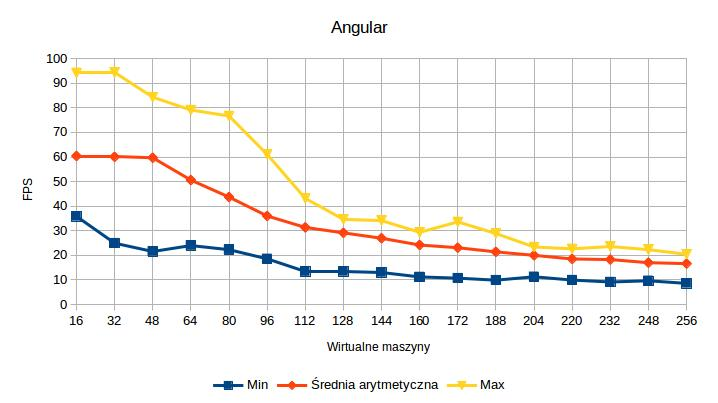
\includegraphics[width=\textwidth]{angular-fps.jpg}
  \caption{Angular - klatki na sekundę (FPS)}
  \label{fig:angular-fps}
\end{figure}

\begin{table}[]
  \centering
  \resizebox{\textwidth}{!}{%
  \begin{tabular}{@{}lllllllllllllllll@{}}
  \toprule
  Wirtualne maszyny      & 16       & 32       & 48       & 64      & 80      & 96      & 112     & 128     & 144     & 160     & 176     & 192     & 208     & 224     & 240     & 256     \\ \midrule
  Min                    & 32.2518  & 23.1401  & 28.3471  & 21.7202 & 21.8790 & 15.8836 & 12.8972 & 12.9643 & 13.9418 & 12.2266 & 11.5253 & 10.7533 & 11.1888 & 10.1081 & 10.7260 & 8.8891  \\
  Średnia arytmetyczna  & 60.5918  & 60.3262  & 59.6180  & 50.9316 & 43.3836 & 35.5747 & 33.2678 & 28.5164 & 27.0781 & 25.0763 & 23.5018 & 22.0219 & 20.5411 & 19.3482 & 18.8703 & 16.9955 \\
  Percentyl 50\%         & 59.5877  & 60.1757  & 59.9592  & 51.8376 & 44.0199 & 36.1024 & 34.3749 & 28.7919 & 27.2250 & 25.3505 & 23.6843 & 22.2479 & 20.6556 & 19.7981 & 19.5557 & 17.5319 \\
  Percentyl 66\%         & 62.1311  & 61.8659  & 60.4376  & 53.2935 & 45.2366 & 37.5530 & 34.9382 & 29.8721 & 28.5968 & 26.6290 & 24.7109 & 23.4318 & 21.4869 & 20.2282 & 19.9465 & 17.9443 \\
  Percentyl 75\%         & 63.7877  & 63.1712  & 60.7497  & 54.2241 & 45.8421 & 38.1913 & 35.2336 & 30.5979 & 29.2287 & 27.0541 & 25.4272 & 23.8158 & 22.1293 & 20.4956 & 20.1284 & 18.1858 \\
  Percentyl 80\%         & 64.7291  & 64.1313  & 61.1995  & 54.8035 & 46.1425 & 38.5253 & 35.3995 & 30.9732 & 29.4516 & 27.2450 & 25.6364 & 23.9785 & 22.3140 & 20.6535 & 20.2388 & 18.3550 \\
  Percentyl 90\%         & 68.2967  & 66.8896  & 62.7156  & 56.1640 & 46.8296 & 39.2912 & 35.8102 & 31.8066 & 29.9016 & 27.6388 & 26.0369 & 24.2990 & 22.6979 & 21.0819 & 20.5036 & 18.6727 \\
  Percentyl 95\%         & 72.6480  & 71.1389  & 63.9468  & 57.0581 & 47.4113 & 39.8359 & 36.0620 & 32.2456 & 30.2014 & 27.9283 & 26.3109 & 24.5248 & 22.9321 & 21.3639 & 20.6744 & 18.8342 \\
  Percentyl 98\%         & 80.3084  & 81.1030  & 67.5995  & 58.0248 & 48.0169 & 40.3714 & 36.3465 & 32.5903 & 30.4609 & 28.2159 & 26.5442 & 24.6840 & 23.1171 & 21.6029 & 20.8385 & 18.9959 \\
  Percentyl 99\%         & 86.7002  & 86.1475  & 69.5846  & 58.5172 & 48.4262 & 40.7448 & 36.5738 & 32.8937 & 30.6157 & 28.3744 & 26.6603 & 24.8028 & 23.2159 & 21.7250 & 20.9275 & 19.0738 \\
  Percentyl 100\%        & 112.5239 & 105.7530 & 115.4468 & 72.5479 & 54.6717 & 54.6001 & 42.1959 & 40.9417 & 39.1527 & 39.8533 & 32.3572 & 26.3463 & 27.7523 & 24.5676 & 23.5266 & 19.7246 \\
  Odchylenie standardowe & 7.1382   & 7.3281   & 4.1700   & 5.0844  & 3.6078  & 3.5785  & 3.0683  & 2.8184  & 2.6217  & 2.5323  & 2.3192  & 2.1870  & 1.8375  & 1.7282  & 1.7944  & 1.7335  \\
  Wariancja              & 50.9533  & 53.7008  & 17.3887  & 25.8511 & 13.0162 & 12.8058 & 9.4146  & 7.9432  & 6.8732  & 6.4124  & 5.3786  & 4.7828  & 3.3766  & 2.9866  & 3.2200  & 3.0049  \\ \bottomrule
  \end{tabular}%
  }
  \caption{AngularJS - klatki na sekundę (FPS)}
  \label{tab:angularjs-fps}
\end{table}

\begin{figure}[ht]
  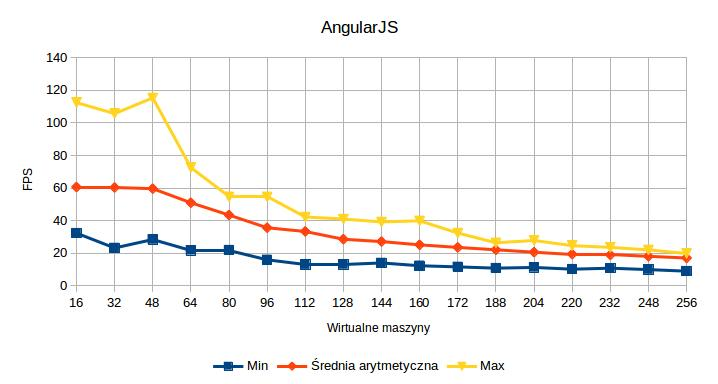
\includegraphics[width=\textwidth]{angularjs-fps.jpg}
  \caption{AngularJS - klatki na sekundę (FPS)}
  \label{fig:angularjs-fps}
\end{figure}

\begin{table}[]
  \centering
  \resizebox{\textwidth}{!}{%
  \begin{tabular}{@{}lllllllllllllllll@{}}
  \toprule
  Wirtualne maszyny      & 16       & 32      & 48      & 64       & 80      & 96      & 112     & 128     & 144      & 160     & 176      & 192     & 208     & 224     & 240     & 256     \\ \midrule
  Min                    & 26.0159  & 20.4052 & 22.9458 & 23.1086  & 24.0877 & 15.6703 & 16.9598 & 15.9637 & 13.9249  & 13.6493 & 10.6918  & 8.8657  & 10.8206 & 10.8158 & 9.7294  & 9.5181  \\
  Średnia arytmetyczna   & 60.7794  & 59.9438 & 58.6511 & 53.8146  & 45.7740 & 38.5110 & 33.6535 & 30.2822 & 29.0721  & 25.9450 & 25.1155  & 23.1510 & 21.8012 & 20.4229 & 19.9175 & 17.7767 \\
  Percentyl 50\%         & 59.6303  & 60.0673 & 59.7979 & 55.0661  & 46.6266 & 39.4446 & 34.3418 & 30.5092 & 29.9742  & 26.0994 & 25.7692  & 23.3498 & 22.1391 & 20.6859 & 20.6505 & 18.0770 \\
  Percentyl 66\%         & 62.9961  & 62.2200 & 60.3500 & 56.6861  & 47.8675 & 41.2235 & 35.4761 & 31.7017 & 30.8166  & 26.9389 & 26.3380  & 24.6130 & 23.0139 & 21.4597 & 21.0735 & 18.7227 \\
  Percentyl 75\%         & 65.6254  & 63.7064 & 61.0389 & 57.6801  & 48.5460 & 41.9076 & 36.0750 & 32.5510 & 31.1808  & 28.0694 & 26.7917  & 25.0583 & 23.4390 & 22.1043 & 21.3079 & 19.2886 \\
  Percentyl 80\%         & 67.2812  & 64.5870 & 61.6371 & 58.3363  & 48.9333 & 42.2779 & 36.3848 & 32.9881 & 31.3529  & 28.4026 & 27.0351  & 25.2704 & 23.6832 & 22.3894 & 21.4436 & 19.5798 \\
  Percentyl 90\%         & 71.9476  & 67.8887 & 63.2351 & 59.8337  & 49.9825 & 43.0182 & 37.1650 & 33.9087 & 31.7460  & 28.9168 & 27.5953  & 25.6865 & 24.1191 & 22.8274 & 21.7391 & 20.0280 \\
  Percentyl 95\%         & 75.9590  & 71.5512 & 65.1848 & 60.9645  & 50.6175 & 43.5635 & 37.6946 & 34.4412 & 31.9826  & 29.2184 & 27.8886  & 25.9336 & 24.3546 & 23.0792 & 21.9274 & 20.3446 \\
  Percentyl 98\%         & 82.3045  & 76.5814 & 68.5307 & 61.9502  & 51.2636 & 44.0160 & 38.1752 & 34.8505 & 32.2227  & 29.4916 & 28.0891  & 26.1465 & 24.5827 & 23.2823 & 22.1048 & 20.5727 \\
  Percentyl 99\%         & 87.5657  & 79.6559 & 70.4821 & 62.4649  & 51.7920 & 44.2811 & 38.4541 & 35.1050 & 32.4265  & 29.6683 & 28.2223  & 26.2812 & 24.6804 & 23.3880 & 22.2247 & 20.7220 \\
  Percentyl 100\%        & 103.1885 & 91.2909 & 76.5814 & 121.8324 & 83.5561 & 65.8458 & 54.0073 & 49.2756 & 156.7890 & 32.5563 & 150.4664 & 29.6033 & 29.9267 & 26.8897 & 26.4208 & 21.5880 \\
  Odchylenie standardowe & 8.6522   & 7.3116  & 6.3986  & 5.9809   & 4.1741  & 4.2367  & 3.3129  & 3.0872  & 3.5115   & 2.5544  & 3.2548   & 2.3106  & 2.1345  & 2.0950  & 2.0087  & 1.9701  \\
  Wariancja              & 74.8604  & 53.4591 & 40.9416 & 35.7713  & 17.4231 & 17.9498 & 10.9750 & 9.5306  & 12.3307  & 6.5250  & 10.5939  & 5.3387  & 4.5560  & 4.3889  & 4.0349  & 3.8814  \\ \bottomrule
  \end{tabular}%
  }
  \caption{mithril.js - klatki na sekundę (FPS)}
  \label{tab:mithril-fps}
\end{table}

\begin{figure}[ht]
  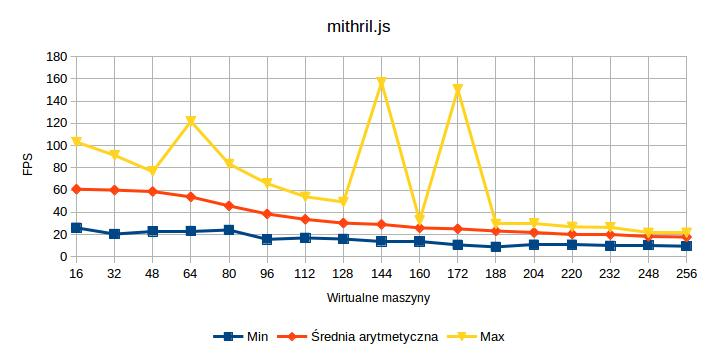
\includegraphics[width=\textwidth]{mithril-fps.jpg}
  \caption{mithril.js - klatki na sekundę (FPS)}
  \label{fig:mithril-fps}
\end{figure}

\begin{table}[]
  \centering
  \resizebox{\textwidth}{!}{%
  \begin{tabular}{@{}lllllllllllllllll@{}}
  \toprule
  Wirtualne maszyny      & 16       & 32       & 48      & 64      & 80      & 96      & 112     & 128     & 144     & 160     & 176     & 192      & 208     & 224     & 240            & 256     \\ \midrule
  Min                    & 28.9519  & 23.3847  & 22.0970 & 20.7822 & 6.2832  & 13.5669 & 10.5009 & 9.8623  & 8.7033  & 7.8844  & 6.4566  & 6.6217   & 5.7962  & 4.6042  & 4.4336         & 4.2413  \\
  Średnia arytmetyczna   & 62.9361  & 55.3910  & 37.8894 & 31.8319 & 25.2395 & 21.3654 & 18.5916 & 16.6169 & 14.9217 & 13.4915 & 12.3384 & 11.5802  & 10.4157 & 9.7899  & 9.3280 & 8.5567        \\
  Percentyl 50\%         & 54.9934  & 56.1861  & 38.3966 & 32.2810 & 25.5853 & 21.6755 & 18.8313 & 16.7330 & 15.1190 & 13.6478 & 12.4881 & 11.6892  & 10.5958 & 9.9584  & 9.4335         & 8.7497  \\
  Percentyl 66\%         & 72.3432  & 57.8737  & 39.5601 & 33.0677 & 26.2784 & 22.2311 & 19.2045 & 17.1453 & 15.5039 & 13.9324 & 12.9321 & 12.0090  & 10.8940 & 10.2011 & 9.6507         & 8.9141  \\
  Percentyl 75\%         & 75.5173  & 58.7372  & 39.9616 & 33.4314 & 26.6951 & 22.5347 & 19.7176 & 17.5735 & 15.7570 & 14.1279 & 13.2333 & 12.4103  & 11.1509 & 10.3860 & 9.8269         & 9.0212  \\
  Percentyl 80\%         & 77.8210  & 59.3049  & 40.1574 & 33.6428 & 26.9288 & 22.7149 & 19.9744 & 17.7487 & 15.8738 & 14.2841 & 13.3586 & 12.5400  & 11.3063 & 10.5558 & 9.9983         & 9.1600  \\
  Percentyl 90\%         & 83.6890  & 60.5877  & 40.6141 & 34.1367 & 27.3913 & 23.1530 & 20.2725 & 18.0005 & 16.1296 & 14.7325 & 13.6322 & 12.7241  & 11.5678 & 10.8220 & 10.2408        & 9.4343  \\
  Percentyl 95\%         & 88.7233  & 61.5801  & 40.9635 & 34.4448 & 27.6786 & 23.4280 & 20.4015 & 18.1689 & 16.2933 & 14.9269 & 13.8001 & 12.8360  & 11.7268 & 10.9570 & 10.3772        & 9.5450  \\
  Percentyl 98\%         & 95.0029  & 63.1632  & 41.3462 & 34.7500 & 27.9322 & 23.6423 & 20.5276 & 18.2942 & 16.4330 & 15.1014 & 13.9639 & 12.9401  & 11.8700 & 11.0882 & 10.5007        & 9.6337  \\
  Percentyl 99\%         & 99.6314  & 64.6329  & 41.6337 & 34.9077 & 28.0844 & 23.7287 & 20.6271 & 18.3702 & 16.5033 & 15.1858 & 14.0479 & 13.0195  & 11.9262 & 11.1540 & 10.5432        & 9.6853  \\
  Percentyl 100\%        & 113.6880 & 131.5616 & 84.1538 & 57.8905 & 47.4338 & 30.1368 & 20.9503 & 19.1942 & 17.4883 & 96.3948 & 14.4563 & 154.7988 & 12.0764 & 11.3294 & 123.9311       & 10.5532 \\
  Odchylenie standardowe & 15.1290  & 5.2970   & 2.8767  & 2.2104  & 2.1052  & 1.6748  & 1.5102  & 1.1882  & 1.1727  & 1.7728  & 1.1697  & 2.7269   & 1.0176  & 0.9256  & 2.2324         & 0.7893  \\
  Wariancja              & 228.8858 & 28.0586  & 8.2754  & 4.8858  & 4.4319  & 2.8049  & 2.2807  & 1.4117  & 1.3753  & 3.1429  & 1.3682  & 7.4357   & 1.0354  & 0.8568  & 4.9838         & 0.6230  \\ \bottomrule
  \end{tabular}%
  }
  \caption{React - klatki na sekundę (FPS)}
  \label{tab:react-fps}
\end{table}

\begin{figure}[ht]
  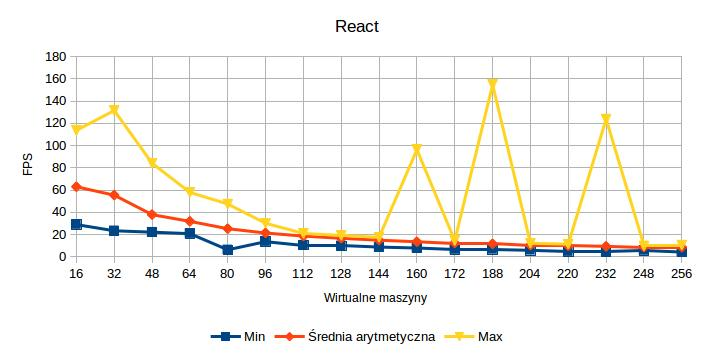
\includegraphics[width=\textwidth]{react-fps.jpg}
  \caption{React - klatki na sekundę (FPS)}
  \label{fig:react-fps}
\end{figure}

\begin{table}[]
  \centering
  \resizebox{\textwidth}{!}{%
  \begin{tabular}{@{}lllllllllllllllll@{}}
  \toprule
  Wirtualne maszyny      & 16      & 32       & 48      & 64      & 80      & 96      & 112     & 128     & 144     & 160     & 176     & 192     & 208     & 224     & 240     & 256     \\ \midrule
  Min                    & 24.3694 & 24.2813  & 26.7766 & 19.1902 & 21.5829 & 2.4832  & 17.1960 & 13.5338 & 12.4321 & 11.0894 & 11.0553 & 9.3312  & 9.1819  & 9.6745  & 8.7072  & 7.5943  \\
  Średnia arytmetyczna   & 60.4745 & 60.0086  & 59.5959 & 48.9094 & 39.7192 & 34.9015 & 30.8042 & 27.1781 & 24.6659 & 23.6055 & 21.2693 & 20.5708 & 18.9126 & 17.4626 & 16.8787 & 15.7355 \\
  Percentyl 50\%         & 59.2768 & 60.3355  & 60.2011 & 50.2285 & 39.9920 & 35.5442 & 31.4653 & 27.4635 & 25.1953 & 24.3191 & 21.6062 & 21.1640 & 19.1655 & 17.7437 & 17.4028 & 16.1998 \\
  Percentyl 66\%         & 61.5953 & 61.1808  & 60.9236 & 51.5172 & 41.4938 & 36.4193 & 32.2103 & 28.3825 & 26.0071 & 24.8954 & 22.2430 & 21.6591 & 19.7593 & 18.2979 & 17.8862 & 16.6085 \\
  Percentyl 75\%         & 63.2511 & 61.8659  & 61.4553 & 52.2521 & 42.3711 & 36.9645 & 32.6755 & 29.0867 & 26.4781 & 25.1769 & 22.7754 & 21.9568 & 20.2992 & 18.7273 & 18.1528 & 16.8245 \\
  Percentyl 80\%         & 65.9979 & 62.2665  & 62.0578 & 52.7065 & 42.8798 & 37.2717 & 32.9587 & 29.4898 & 26.7437 & 25.3537 & 23.0910 & 22.1641 & 20.5639 & 18.9822 & 18.2705 & 16.9471 \\
  Percentyl 90\%         & 70.5766 & 63.3152  & 63.4437 & 53.8735 & 43.9020 & 38.0416 & 33.6281 & 30.3435 & 27.3748 & 25.7539 & 23.6513 & 22.5175 & 21.0146 & 19.5221 & 18.6836 & 17.1984 \\
  Percentyl 95\%         & 73.5727 & 64.8424  & 64.4205 & 54.6538 & 44.5851 & 38.5015 & 34.1425 & 30.8814 & 27.7285 & 26.0017 & 23.9006 & 22.7350 & 21.2504 & 19.7632 & 18.9165 & 17.3859 \\
  Percentyl 98\%         & 76.9941 & 74.3660  & 66.2076 & 55.6421 & 45.3844 & 38.8697 & 34.6320 & 31.3470 & 27.9877 & 26.2323 & 24.1260 & 22.9163 & 21.4749 & 19.9577 & 19.1197 & 17.5630 \\
  Percentyl 99\%         & 80.1989 & 79.4976  & 67.5493 & 56.1356 & 45.8610 & 39.1190 & 34.9162 & 31.6196 & 28.1539 & 26.3532 & 24.2460 & 23.0012 & 21.6043 & 20.0329 & 19.2315 & 17.6451 \\
  Percentyl 100\%        & 98.7069 & 101.6777 & 77.6880 & 81.3273 & 56.8893 & 56.5259 & 39.2866 & 33.8868 & 36.6865 & 28.9084 & 26.5048 & 28.8085 & 27.5475 & 21.9135 & 22.2573 & 20.5132 \\
  Odchylenie standardowe & 6.9269  & 5.1959   & 4.5495  & 5.1628  & 3.6607  & 3.1499  & 2.8411  & 2.6786  & 2.4695  & 2.2950  & 2.1045  & 1.9651  & 1.8464  & 1.7407  & 1.7701  & 1.4711  \\
  Wariancja              & 47.9819 & 26.9972  & 20.6979 & 26.6544 & 13.4007 & 9.9218  & 8.0717  & 7.1748  & 6.0986  & 5.2669  & 4.4289  & 3.8614  & 3.4090  & 3.0302  & 3.1334  & 2.1642  \\ \bottomrule
  \end{tabular}%
  }
  \caption{Vue.js - klatki na sekundę (FPS)}
  \label{tab:vue-fps}
\end{table}

\begin{figure}[ht]
  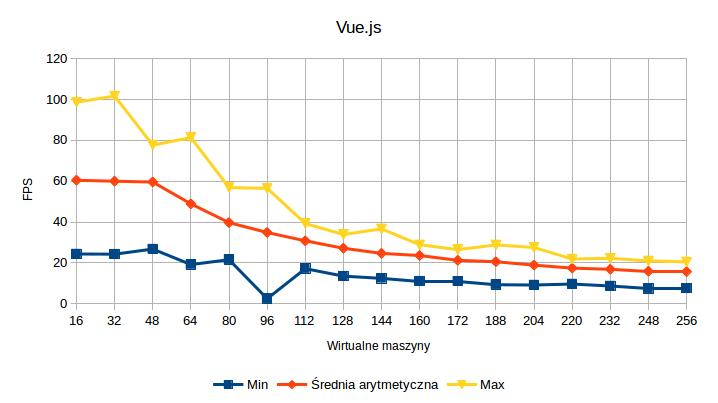
\includegraphics[width=\textwidth]{vue-fps.jpg}
  \caption{Vue.js - klatki na sekundę (FPS)}
  \label{fig:vue-fps}
\end{figure}

\subsection{Badania wydajności pamięciowej}

Wydajność pamięciowa mierzona została na podstawie minimalnej wielkości pamięci zaalokowanej na stercie (ang. \emph{heap}), przy której aplikacja była w stanie poprawnie funkcjonować.

Tablice \ref{tab:angular-heap}, \ref{tab:angularjs-heap}, \ref{tab:mithril-heap}, \ref{tab:react-heap}, \ref{tab:vue-heap} przedstawiają minimalny rozmiar sterty w zależności od liczby wirtualnych maszyn dla poszczególnych bibliotek.

\begin{table}[]
  \centering
  \resizebox{\textwidth}{!}{%
  \begin{tabular}{@{}llllllllllllllllll@{}}
  \toprule
  Wirtualne maszyny                 & 16         & 32         & 48         & 64         & 80         & 96         & 112        & 128        & 144        & 160        & 176        & 192        & 208        & 224        & 240        & 256        &  \\ \midrule
  Minimalny rozmiar sterty {[}KB{]} & 27616.4135 & 27904.7750 & 28837.2877 & 29145.9789 & 29842.1646 & 30206.0723 & 29421.7389 & 31079.5915 & 30698.3522 & 31871.6344 & 32047.2940 & 32548.6094 & 33361.6876 & 33537.3595 & 34001.3173 & 35563.6187 &  \\ \bottomrule
  \end{tabular}%
  }
  \caption{Angular - minimalny rozmiar sterty}
  \label{tab:angular-heap}
\end{table}

\begin{table}[]
  \centering
  \resizebox{\textwidth}{!}{%
  \begin{tabular}{@{}lllllllllllllllll@{}}
  \toprule
  Wirtualne maszyny        & 16         & 32         & 48         & 64         & 80         & 96         & 112        & 128        & 144        & 160        & 176        & 192        & 208        & 224        & 240        & 256        \\ \midrule
  Minimalny rozmiar sterty [KB] & 24673.3543 & 22853.7092 & 25179.1871 & 26652.4256 & 26647.9803 & 26334.2587 & 26549.8688 & 27819.5247 & 27761.2876 & 28738.2432 & 29175.9008 & 29520.0147 & 30713.3663 & 30983.3087 & 32922.8489 & 31867.9627 \\ \bottomrule
  \end{tabular}%
  }
  \caption{AngularJS - minimalny rozmiar sterty}
  \label{tab:angularjs-heap}
\end{table}

\begin{table}[]
  \centering
  \resizebox{\textwidth}{!}{%
  \begin{tabular}{@{}llllllllllllllllll@{}}
  \toprule
  Wirtualne maszyny                 & 16         & 32         & 48         & 64         & 80         & 96         & 112        & 128        & 144        & 160        & 176        & 192        & 208        & 224        & 240        & 256        &  \\ \midrule
  Minimalny rozmiar sterty {[}KB{]} & 18669.9500 & 19538.4679 & 20058.1274 & 20743.9502 & 20146.2873 & 21003.1107 & 22878.2463 & 24677.9818 & 23188.6286 & 26401.9418 & 26450.3174 & 27740.6897 & 27301.4939 & 27975.4485 & 29538.7823 & 29005.0794 &  \\ \bottomrule
  \end{tabular}%
  }
  \caption{mithril.js - minimalny rozmiar sterty}
  \label{tab:mithril-heap}
\end{table}

\begin{table}[]
  \centering
  \resizebox{\textwidth}{!}{%
  \begin{tabular}{@{}llllllllllllllllll@{}}
  \toprule
  Wirtualne maszyny                 & 16         & 32         & 48         & 64         & 80         & 96         & 112        & 128        & 144        & 160        & 176        & 192        & 208        & 224        & 240        & 256        &  \\ \midrule
  Minimalny rozmiar sterty {[}KB{]} & 16593.4993 & 16373.5054 & 17214.0475 & 18794.2027 & 18682.6790 & 20964.7949 & 22769.6739 & 22693.9105 & 22893.5562 & 24570.8424 & 24548.7582 & 26200.6102 & 26304.3926 & 26482.7452 & 27468.6351 & 28057.6440 &  \\ \bottomrule
  \end{tabular}%
  }
  \caption{React - minimalny rozmiar sterty}
  \label{tab:react-heap}
\end{table}

\begin{table}[]
  \centering
  \resizebox{\textwidth}{!}{%
  \begin{tabular}{@{}llllllllllllllllll@{}}
  \toprule
  Wirtualne maszyny                 & 16         & 32         & 48         & 64         & 80         & 96         & 112        & 128        & 144        & 160        & 176        & 192        & 208        & 224        & 240        & 256        &  \\ \midrule
  Minimalny rozmiar sterty {[}KB{]} & 13623.7795 & 14438.9178 & 15281.2367 & 15453.4944 & 17270.8171 & 18658.5004 & 19278.2128 & 19529.2375 & 19932.1830 & 21786.8748 & 22258.4797 & 22251.7257 & 23164.2905 & 25416.1206 & 24377.4772 & 25230.7092 &  \\ \bottomrule
  \end{tabular}%
  }
  \caption{Vue.js - minimalny rozmiar sterty}
  \label{tab:vue-heap}
\end{table}

\section{Porównanie wyników i wnioski}

\subsection{Wydajność czasowa}

\begin{figure}[ht]
  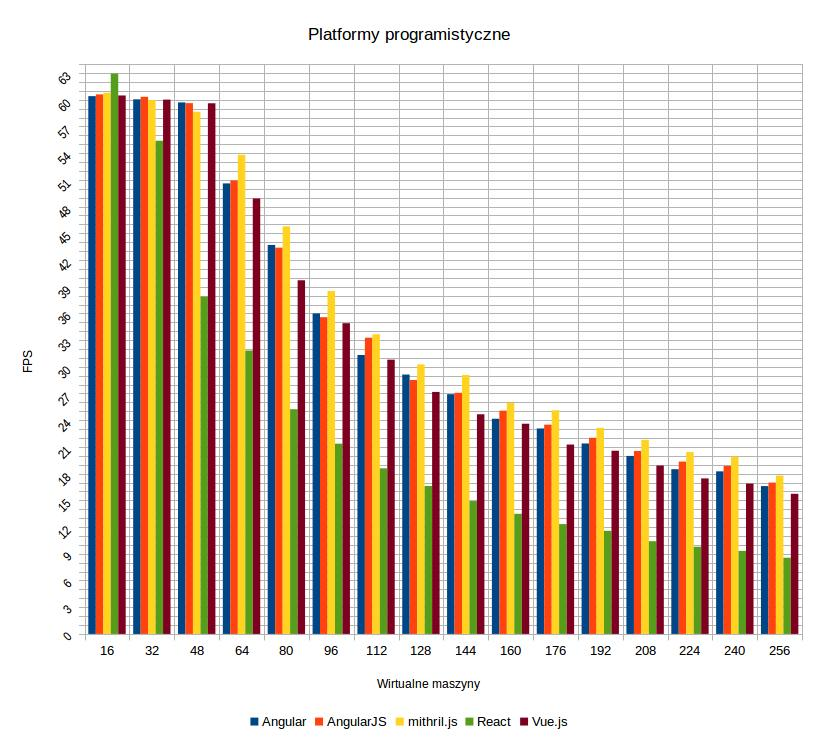
\includegraphics[width=\textwidth]{frameworks-fps.jpg}
  \caption{Platformy programistyczne - klatki na sekundę (FPS)}
  \label{fig:frameworks-fps}
\end{figure}

Analizując rysunek \ref{fig:frameworks-fps} przedstawiający porównanie ilości klatek na sekundę (im więcej tym lepiej) w zależności od wirtualnych maszyn jednoznacznie najlepiej wypada platforma programistyczna \emph{mithril.js}. Na kolejnych miejscach plasują się platformy \emph{AngularJS} oraz \emph{Angular}. Co ciekawe następca \emph{AngularJS} wypadł gorzej od swojego poprzednika. Na przedostatnim miejscu uplasował się \emph{Vue.js} odbiegający od triumfatora średnio o kilka klatek na sekundę. Zdecydowanie najgorzej wypadł \emph{React} zdecydowanie odbiegając od reszty. Może to być przyczyną nieoptymalnej implementacji dla danego scenariusza testowego, była ona jednak oparta na oficjalnej dokumentacji biblioteki \emph{React} z uwzględnieniem wszelkich informacji o potencjalnych, popularnych błędach implementacyjnych. 

Biblioteki implementujące mechanizm wirtualnego obiektowego modelu dokumentu nie osiągnęły zdecydowanie lepszych wyników od bibliotek pozbawionych tego mechanizmu. Co prawda zwycięzcą został \emph{mithril.js}, lecz odpowiednio na drugim i trzecim miejscu uplasowały się biblioteki bez tego mechanizmu czyli \emph{AngularJS} oraz \emph{Angular}.

\subsection{Wydajność pamięciowa}

\begin{figure}[ht]
  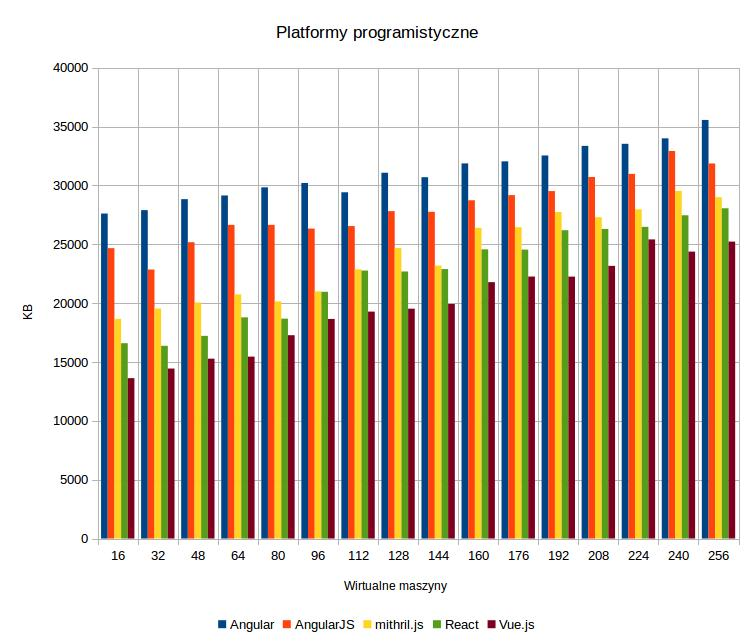
\includegraphics[width=\textwidth]{frameworks-heap.jpg}
  \caption{Platformy programistyczne - minimalny rozmiar sterty}
  \label{fig:frameworks-heap}
\end{figure}

Dokonując analizy rysunku \ref{fig:frameworks-heap} przestawiającego minimalny rozmiar sterty zarezerwowanej przez platformy programistyczne w zależności od liczby wirtualnych maszyn wyraźnie zauważyć można, iż najgorzej wypadły platformy z rodziny \emph{Angular} zdecydowanie odbiegając od swoich konkurentów. Pośrodku uplasowała się biblioteka \emph{mithril.js}, która osiągneła najlepsze wyniki przy badaniu wydajności czasowej. \emph{React} zajął drugie miejsce, natomiast najmniejsze zużycie pamięci wykazała biblioteka \emph{Vue.js}.

\section{Podsumowanie}

Celem pracy było porównanie pięciu platform programistycznych służących do tworzenia aplikacji internetowych. Porównanie zostało przeprowadzone zostało pod kątem wydajności czasowej oraz pamięciowej. Uzyskane wyniki mogą pomoć programistom zadecydować z jakiej biblioteki skorzystać jeśli ważnym kryterium wyboru jest wydajność.

Wyniki badań pokazały, że bardzo ciekawą propozycją jest platforma programistyczna \emph{mithril.js}, która pomimo tego, że nie jest najpopularniejszą biblioteką to uzyskała bardzo dobre wyniki w przeprowadzonych badaniach. 

Niepokojący jest fakt, iż następca \emph{AngularJS} osiągnął gorsze wyniki od swojego poprzednika zarówno w przypadku wydajności czasowej jak i pamięciowej. Dodatkowo rozmiar platformy \emph{Angular} jest zdecydowanie większy od swoich konkurentów co może wpływać negatywnie na działanie u użytkowników posiadających wolniejsze połączenie internetowe.

Biblioteka \emph{Vue.js} posiada wiele nawiązań do \emph{AngularJS} jednak znacznie uproszczonych co powoduje, że z biblioteki korzysta się bardzo wygodnie. Wyniki wydajności czasowej jednak nie zachwycają i mogą skierować uwagę programistów w stronę konkurentów.

Bardzo zagadkowe są wyniki wydajności czasowej osiągnięte przez bardzo popularną bibliotekę \emph{React}. Szersze zbadanie tego problemu może być dobrą propozycją do analizy w ramach dalszego rozwoju tematu pracy.

Istnieje wiele różnych kierunków, w których temat pracy magisterkiej może być dalej rozwijany. Poniżej przedstawiono niektóre z nich.

\begin{itemize}
  \item zbadanie kolejnych platform programistycznych,
  \item przygotowanie kolejnych scenariuszy testowych, które będą w stanie wykazać sytuacje, w których na przykład lepsze okażą się biblioteki implementujące mechanizm wirtualnego obiektowego modelu dokumentu,
  \item wykonanie badań w środowisku innej przeglądarki internetowej również udostępniającej informacje na temat wydajności za pomocą odpowiednich interfejsów. Potencjalnym kandydatem może być przeglądarka \emph{Mozilla Firefox} \cite{firefox},
  \item dalsza automatyzacja procesu zbierania danych oraz ich analizy.
\end{itemize}

\begin{thebibliography}{11}
  \bibitem{react}
    \url https://reactjs.org/
  \bibitem{angularjs}
    \url https://angularjs.org/
  \bibitem{angular}
    \url https://angular.io/
  \bibitem{mithril.js}
    \url https://mithril.js.org
  \bibitem{vue.js}
    \url https://vuejs.org/
  \bibitem{ftrace}
    \url{https://www.kernel.org/doc/Documentation/trace/ftrace.txt}
  \bibitem{etw}
    \url{https://msdn.microsoft.com/pl-pl/library/windows/desktop/bb968803(v=vs.85).aspx}
  \bibitem{battor}
    \url{https://github.com/aschulm/battor}
  \bibitem{milligram}
    \url{http://milligram.io/}
  \bibitem{node.js}
    \url{http://nodejs.org/}
  \bibitem{v8}
    \url{https://github.com/v8/v8}
  \bibitem{npm}
    \url{https://www.npmjs.com/}
  \bibitem{yarn}
    \url{https://yarnpkg.com/}
  \bibitem{es2016}
    \url{https://www.ecma-international.org/ecma-262/7.0/}
  \bibitem{express}
    \url{https://expressjs.com/}
  \bibitem{selenium}
    \url{https://github.com/SeleniumHQ/selenium}
  \bibitem{wd}
    \url{https://github.com/admc/wd}
  \bibitem{spdy}
    \url{http://dev.chromium.org/spdy/}
  \bibitem{w3c}
    \url{https://www.w3.org/}
  \bibitem{w3c-rec-html51}
    \url{https://www.w3.org/TR/html51/}
  \bibitem{w3c-rec-css3-background}
    \url{https://www.w3.org/TR/css3-background/}
  \bibitem{w3c-rec-css3-box}
    \url{https://www.w3.org/TR/css3-box/}
  \bibitem{w3c-rec-css3-cascade}
    \url{https://www.w3.org/TR/css-cascade-3/}
  \bibitem{w3c-rec-css3-color}
    \url{https://www.w3.org/TR/css3-color/}
  \bibitem{w3c-rec-css3-content}
    \url{https://www.w3.org/TR/css-content-3/}
  \bibitem{w3c-rec-css3-fonts}
    \url{https://www.w3.org/TR/css-fonts-3/}
  \bibitem{w3c-rec-css3-gcpm}
    \url{https://www.w3.org/TR/css-gcpm-3/}
  \bibitem{w3c-rec-css3-template}
    \url{https://www.w3.org/TR/css-template-3/}
  \bibitem{w3c-rec-css3-mediaqueries}
    \url{https://www.w3.org/TR/css3-mediaqueries/}
  \bibitem{w3c-rec-css3-multicol}
    \url{https://www.w3.org/TR/css3-multicol/}
  \bibitem{w3c-rec-css3-page}
    \url{https://www.w3.org/TR/css3-page/}
  \bibitem{w3c-rec-css3-selectors}
    \url{https://www.w3.org/TR/css3-selectors/}
  \bibitem{w3c-rec-css3-ui}
    \url{https://www.w3.org/TR/css-ui-3/}
  \bibitem{w3c-rec-dom-level-1}
    \url{https://www.w3.org/TR/DOM-Level-1/}
  \bibitem{w3c-rec-dom-level-2}
    \url{https://www.w3.org/TR/DOM-Level-2/}
  \bibitem{w3c-rec-dom-level-3-core}
    \url{https://www.w3.org/TR/DOM-Level-3-Core/}
  \bibitem{w3c-rec-dom-level-3-ls}
    \url{https://www.w3.org/TR/DOM-Level-3-LS/}
  \bibitem{w3c-rec-dom-level-3-xpath}
    \url{https://www.w3.org/TR/DOM-Level-3-XPath/}
  \bibitem{w3c-rec-dom-level-3-views}
    \url{https://www.w3.org/TR/DOM-Level-3-Views/}
  \bibitem{w3c-rec-dom-level-3-requirements}
    \url{https://www.w3.org/TR/DOM-Requirements/}
  \bibitem{w3c-rec-dom-level-3-val}
    \url{https://www.w3.org/TR/DOM-Level-3-Val/}
  \bibitem{rfc2616}
    \url{https://www.ietf.org/rfc/rfc2616}
  \bibitem{rfc2660}
    \url{https://www.ietf.org/rfc/rfc2660}
  \bibitem{rfc7540}
    \url{https://www.ietf.org/rfc/rfc7540}
  \bibitem{chrome}
    \url{https://www.google.pl/chrome/browser/desktop/index.html}
  \bibitem{chrome-devtools}
    \url{https://developers.google.com/web/tools/chrome-devtools/}
  \bibitem{trace-event-format}
    \url{https://docs.google.com/document/d/1CvAClvFfyA5R-PhYUmn5OOQtYMH4h6I0nSsKchNAySU/edit}
  \bibitem{json}
    \url{http://www.json.org/}
  \bibitem{firefox}
    \url{https://www.mozilla.org/pl/firefox/}
\end{thebibliography}

\end{document}
